\chapter{Implementación}

Este capítulo tratará sobre las herramientas utilizadas para la implementación y planificación, así como los distintos algoritmos que se emplearán para realizar la simulación. Además, se detallará el diseño de los \textit{blueprints} y se describirán las reglas que seguirá el algoritmo de navegación.

\section{Herramientas utilizadas}

En el desarrollo del proyecto se utilizará \verb|git| para el control de versiones del proyecto.
%  y se almacenará en un repositorio de GitHub. 

\bigskip

Para el modelado, texturizado de los distintos objetos de la aplicación y el \textit{rigging} de los vehículos se utilizará Blender\cite{blender}.

\begin{figure}[H]
    \centering
    
\includegraphics[width=0.6\textwidth]{imagenes/blender-logo.png}
    \caption{Logotipo de Blender\cite{blender-logo}.}
    \label{fig:logoblender}
\end{figure}

Asimismo, para la creación y modificación de las texturas se utilizará GIMP\cite{gimp}.

\begin{figure}[H]
    \centering
    
\includegraphics[width=0.3\textwidth]{imagenes/gimp-logo.png}
    \caption{Logotipo de GIMP\cite{gimp}.}
    \label{fig:logogimp}
\end{figure}

\bigskip

% En cuanto a herramientas para la planificación, se hará uso de la herramienta \planApp para llevar un control de las Historias de Usuario que se realizan y pendientes en cada Sprint.
En lo que respecta a herramientas de planificación, se utilizará \planApp para llevar un control de las historias de usuario realizadas y pendientes en cada sprint. Además, se utilizará el \textit{power-up} ``Card Priority Badge'' de ``Kryl Solutions'' para poder anotar la prioridad de cada historia de usuario. Asimismo, se hará uso del \textit{power-up} ``Agile Tools by Corrello'' para poder tener estimaciones en las historias de usuario.

% foto de \planApp
% \begin{figure}[H]
%     \centering
%     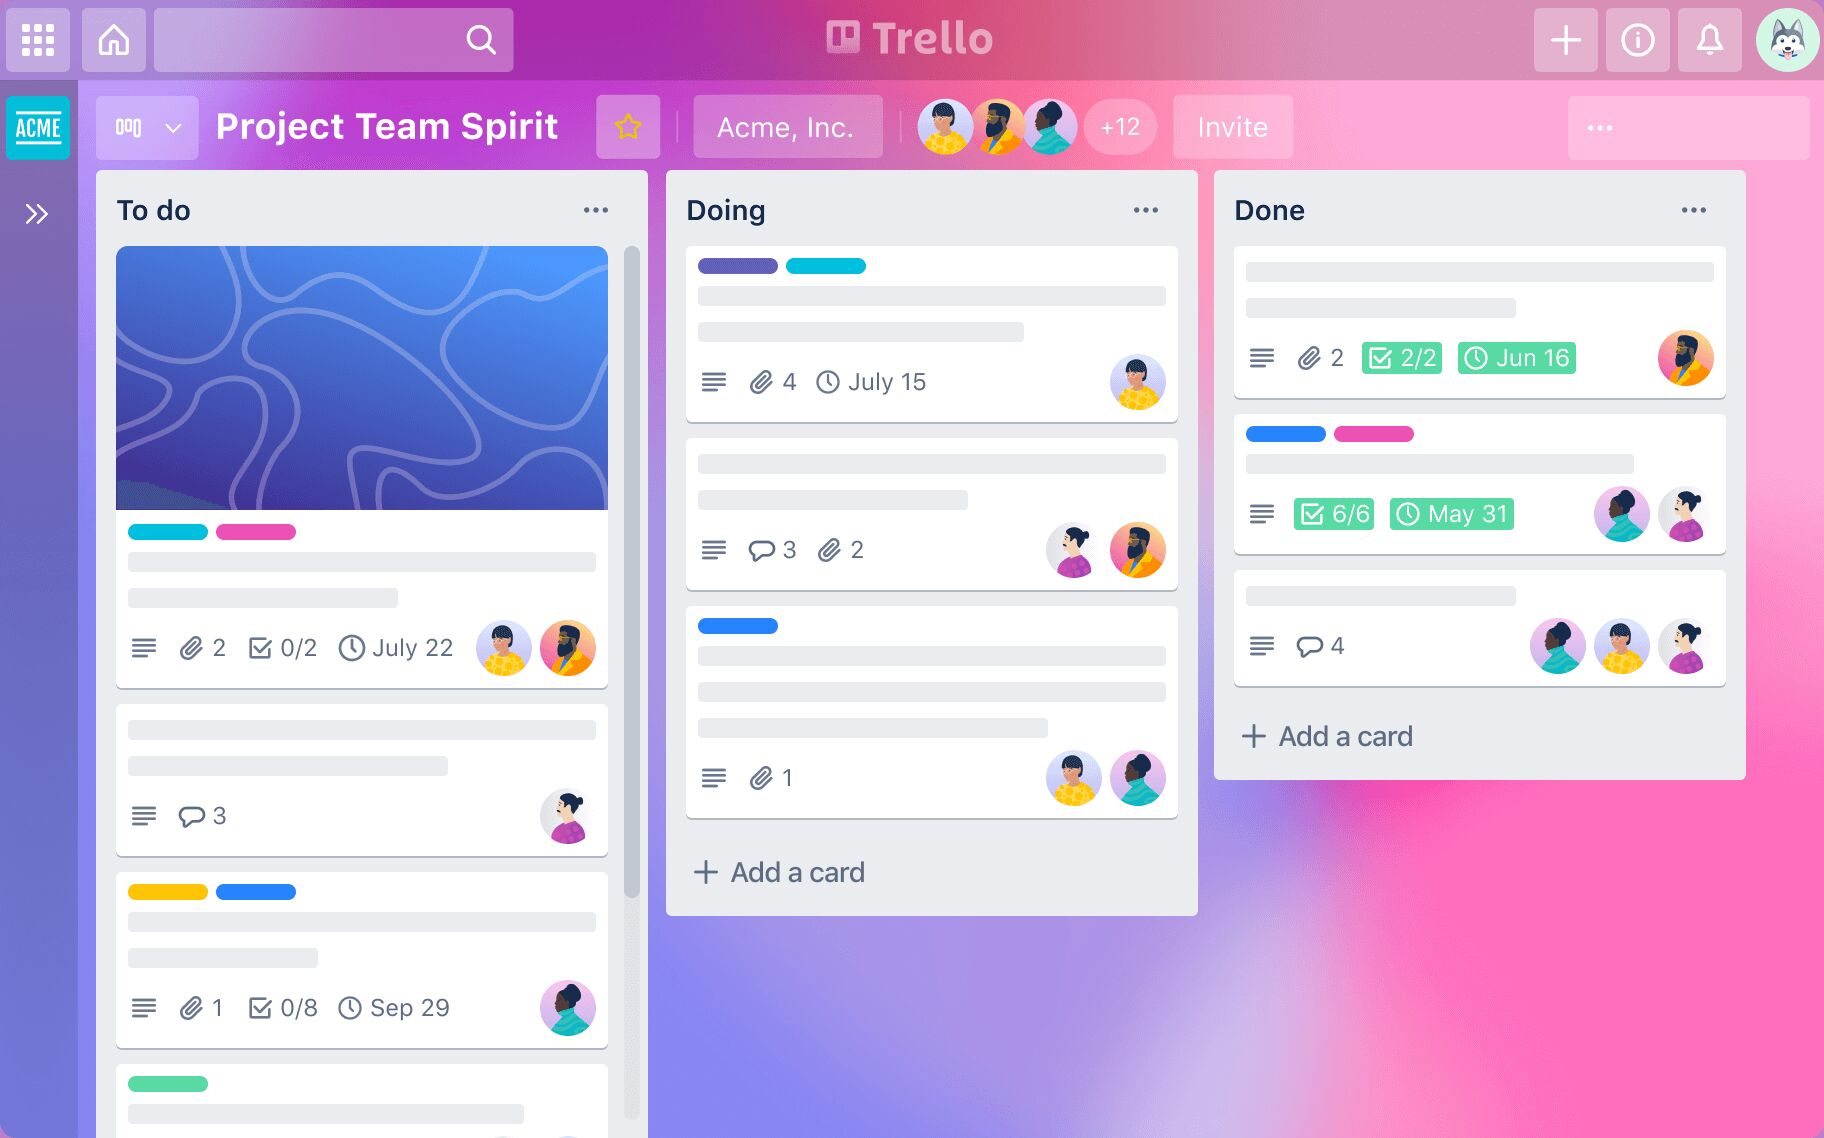
\includegraphics[width=\textwidth]{imagenes/converted/trello.jpg}
%     \caption{Tablero de ejemplo de Trello\cite{tablero-trello}.}
% \end{figure}
\begin{figure}[H]
    \centering
    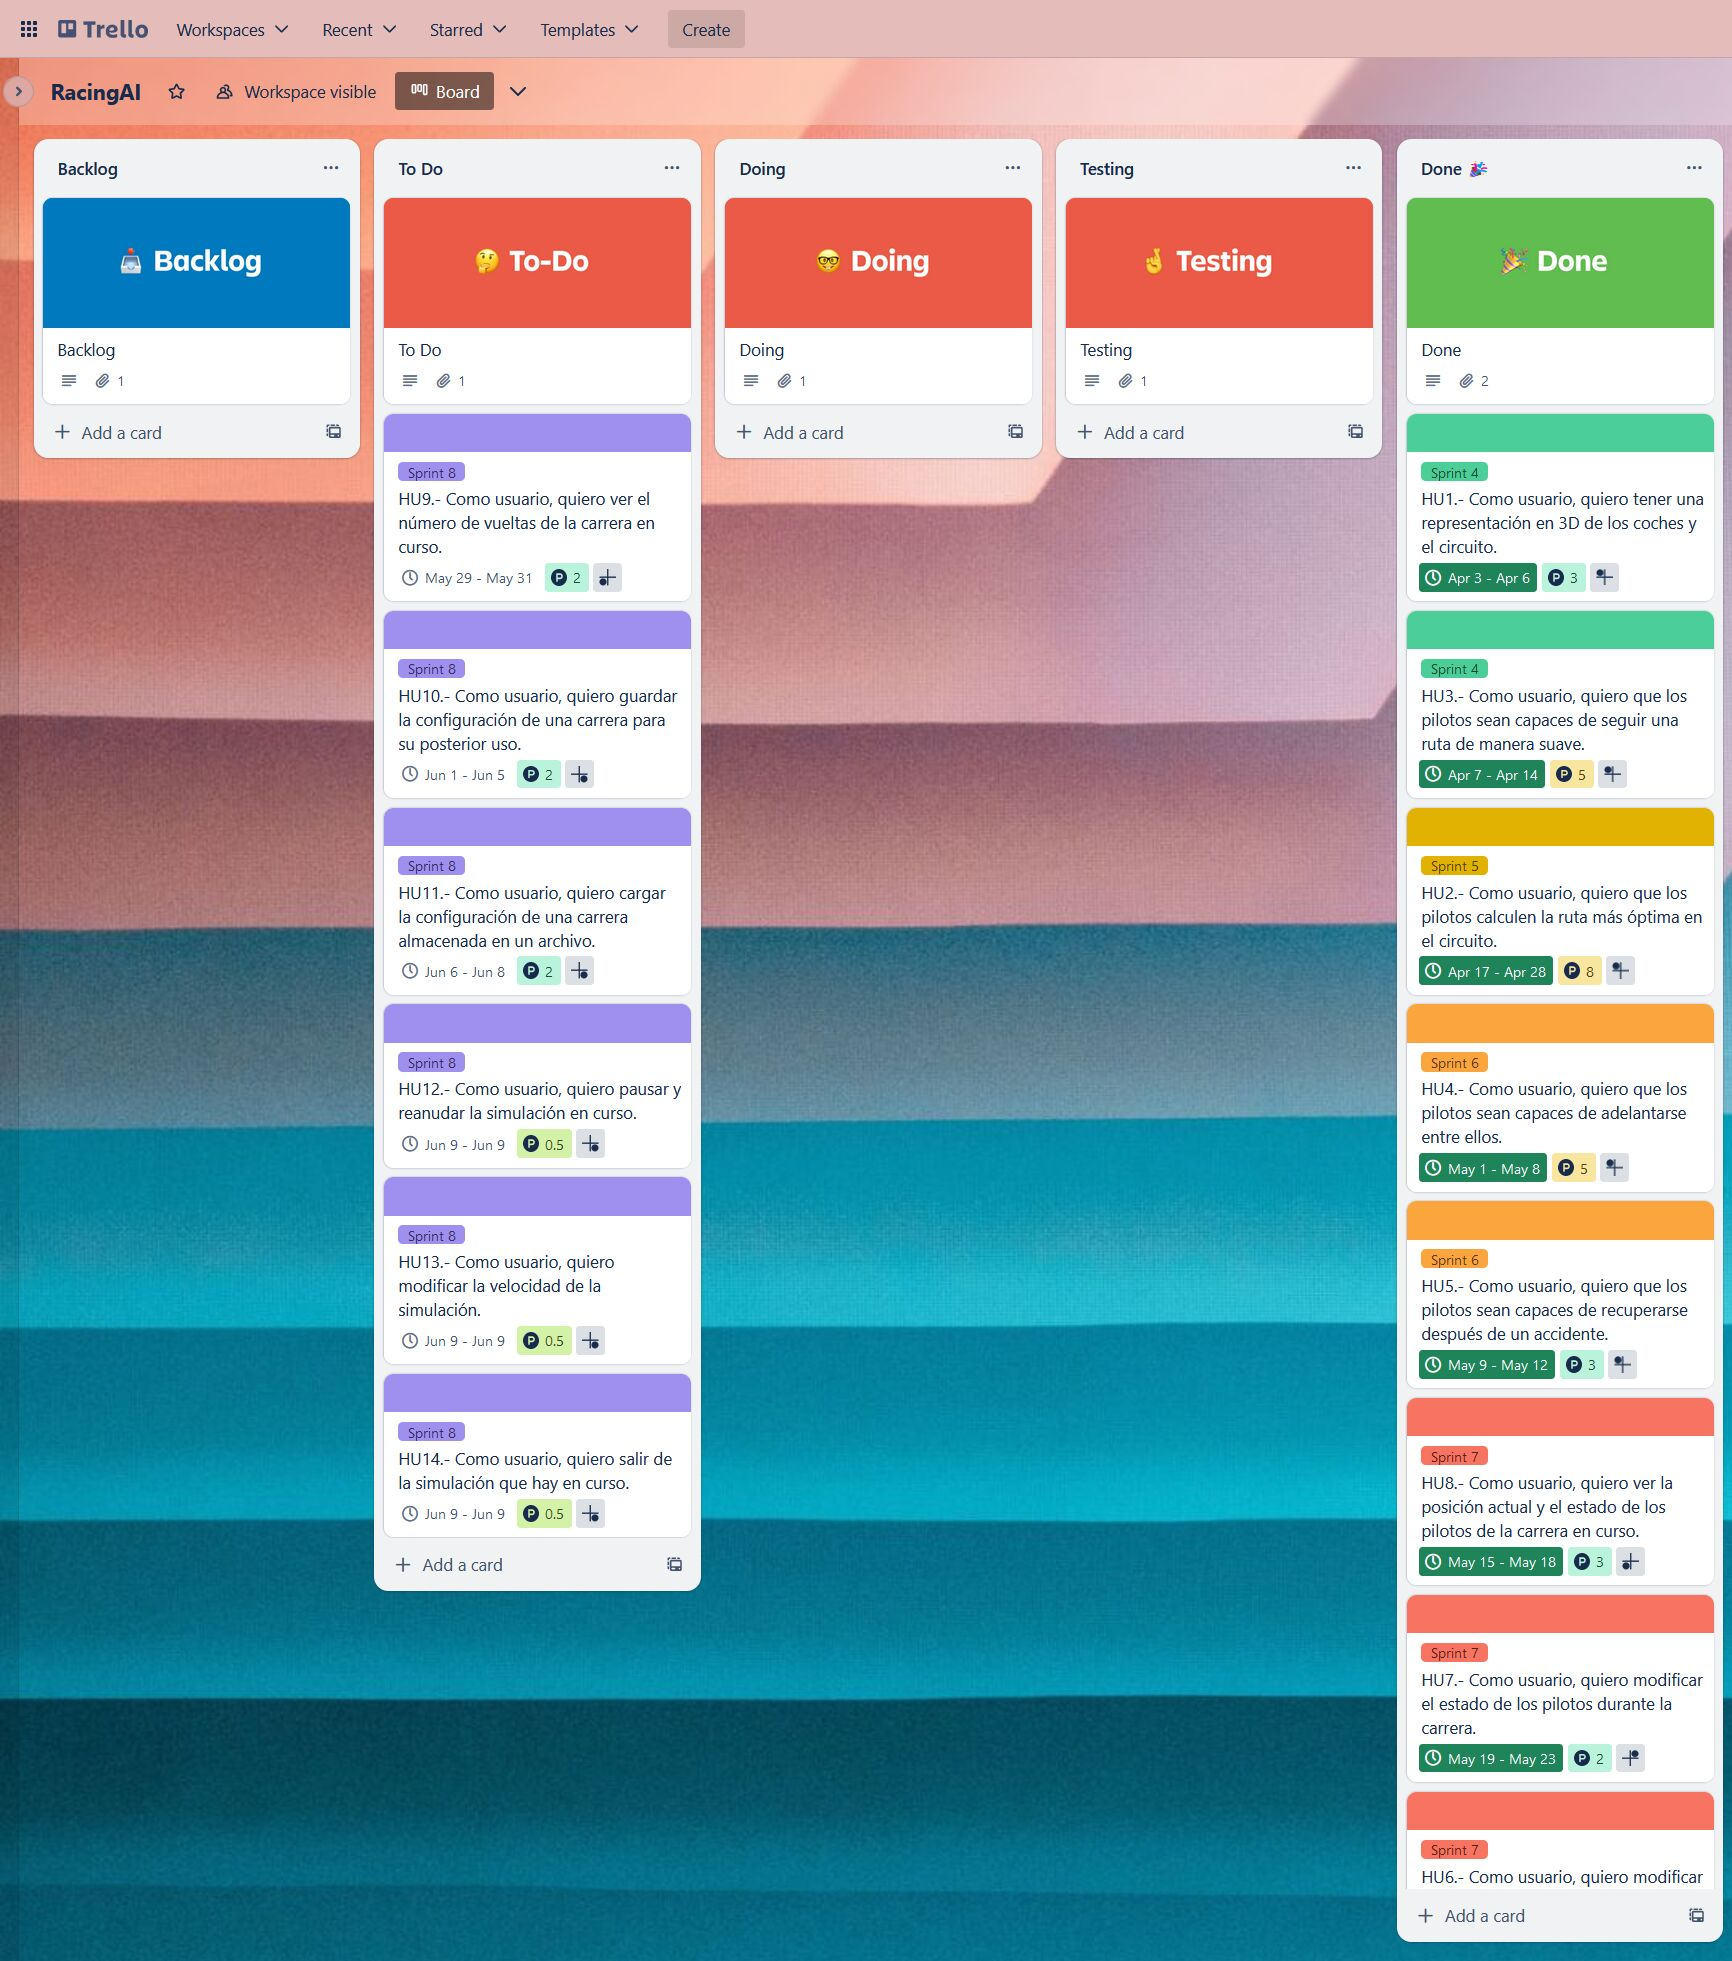
\includegraphics[width=\textwidth]{imagenes/converted/trello-mio.jpg}
    \caption{Tablero utilizado para el proyecto.}
\end{figure}

\newpage

\section{Glosario de términos de Unreal}
\label{sec:terminosunreal}
Esta sección es utilizada como una breve explicación de las palabras utilizadas referentes a Unreal Engine en este capítulo:

\begin{itemize}
    \item \textbf{Blueprint: }Forma visual de implementar lógica en el videojuego mediante el uso de nodos y aristas. Permiten programar sin necesidad de conocer la API en C++.
    \item \textbf{Evento (Event): }Acción o suceso que ocurre durante el juego y que puede desencadenar acciones o comportamiento. Los eventos pueden estar relacionados con el jugador, colisión entre objetos, etc.
    \item \textbf{Actor: }Es un objeto del mundo que puede tener presencia física, implementar comportamiento específico y ser creados en tiempo de ejecución. A grandes rasgos son una clase que pueden tener mallas de polígonos almacenadas.
    \item \textbf{Peón: }Tipo de actor que puede ser controlado directamente por el jugador. Por lo general, los peones representan personajes jugables en el juego.
    \item \textbf{Event ActorBeginOverlap: }Evento utilizado cuando un actor se superpone con otro actor. Puede ser utilizado para realizar acciones en caso de colisión.
    \item \textbf{Event ActorEndOverlap: }Evento que se activa cuando un actor deja de solaparse con otro. Puede ser utilizado para realizar acciones cuando se active el evento.
    \item \textbf{Event Tick: }Evento que ocurre cada fotograma del videojuego y puede desencadenar acciones. Se utiliza para acciones que necesitan actualizaciones continuas, como la animación, el control del volante y los pedales o el seguimiento de otros objetos.
    \item \textbf{Event Hit: }Evento que se activa cuando un objeto colisiona con otro objeto. Puede utilizarse para realizar acciones específicas cuando ocurre una colisión.
\end{itemize}

\newpage

\section{Algoritmos utilizados}

Voy a dividir en subsecciones los diversos algoritmos que componen la simulación:

\subsection{Algoritmo para el giro del volante del coche}

En el control del volante de los vehículos, correspondiente a HU3 y realizada en el sprint 4, se ha utilizado un controlador PID (\textit{Proportional, Integral} y \textit{Derivative}). Este controlador se utiliza para regular el error de un sistema de manera suave, evitando producir muchas desviaciones mediante el ajuste de tres constantes, una para cada componente del controlador. Cabe destacar que la variable a la que el sistema debe llegar se llama SP (\textit{Set Point}) y el valor actual del sistema se denomina PV (\textit{Process Variable}). 

\bigskip

Para que el controlador funcione bien, es necesario modificar sus tres constantes: 
% Proporcional, Integral y Derivativa. 

\begin{itemize}
    \item \textbf{Proporcional: }Actuará de manera proporcional al error actual, multiplicada por la constante asociada. Si solo se utiliza este componente, el sistema se pasará del SP, haciendo que tenga que volver a corregir, produciendo así demasiadas oscilaciones para llegar al SP. 

    \item \textbf{Integral: }Se encarga de derivar el error con respecto al tiempo, con el objetivo de anular errores residuales e incluso del propio sensor. Por normal general, seguirá pasándose del SP, ya que de esto se encarga la componente derivativa.

    \item \textbf{Derivativa: }Se utiliza para estimar como evolucionará la curva con el tiempo, basándose en su pendiente. Esta componente es la que se encarga de minimizar las oscilaciones, al reducir el efecto del actuador si se acerca demasiado rápido al SP.
\end{itemize}

\bigskip

% foto de la constante
\begin{figure}[H]
\centering
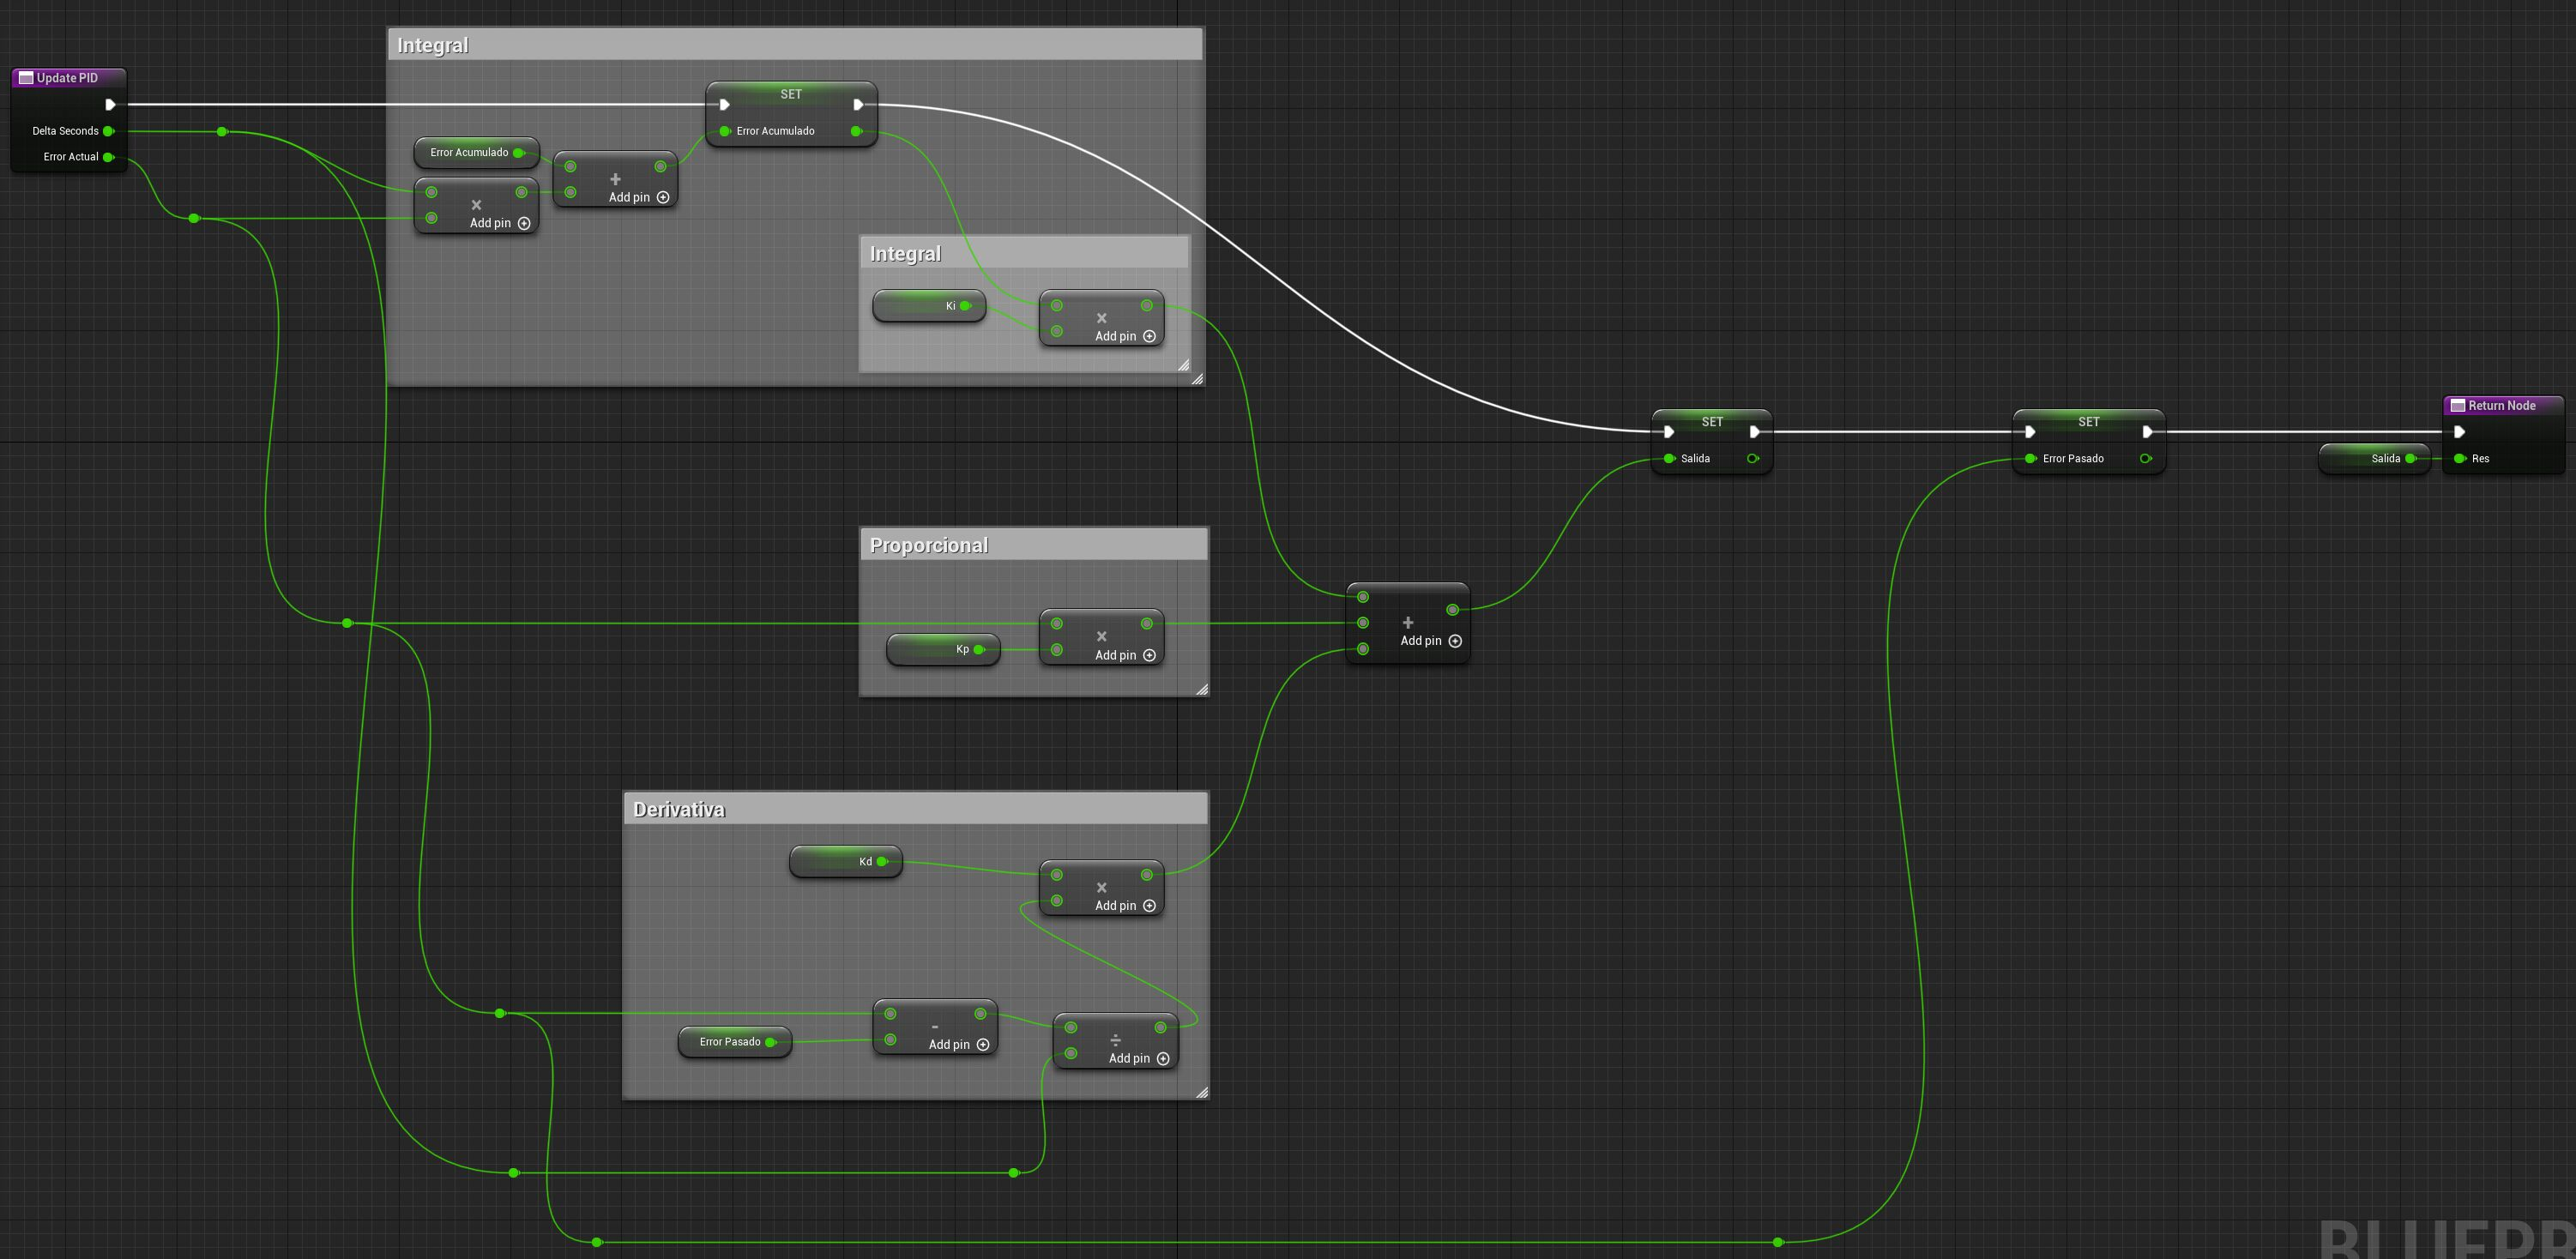
\includegraphics[width=0.83\textwidth]{imagenes/converted/PID-BP.jpg}
\caption{Implementación usando \textit{blueprints} del controlador PID.}
\label{fig:pidbp}
\end{figure}

El rango de valores que pueden tener las variables dependen del sistema al que se aplique. No obstante, todos los valores son números reales positivos, incluyendo el 0, que deshabilita la componente.

\bigskip

Cabe destacar que, en mi caso, el SP es el punto más cercano del coche a la ruta generada, y el error es la distancia del coche a dicho punto.

\begin{figure}[H]
    \centering
    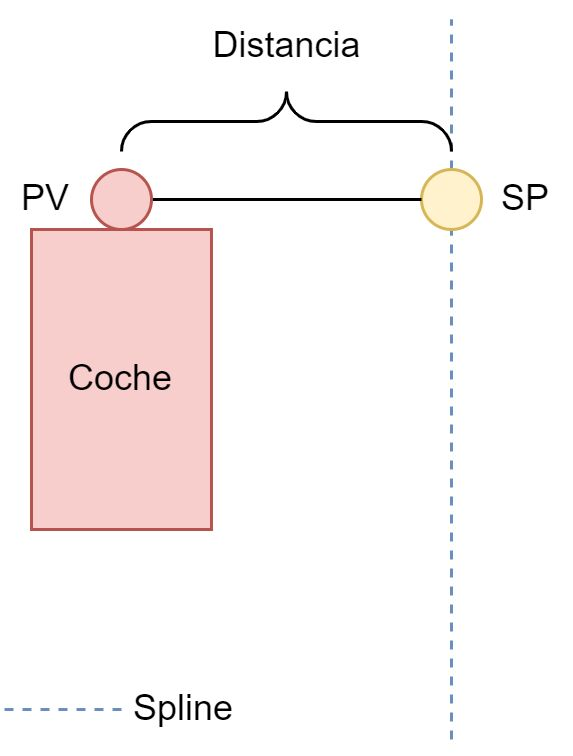
\includegraphics[width=0.4\textwidth]{imagenes/converted/errorPID.jpg}
    \caption{Esquema donde se indica el cálculo de la distancia para el PID.}
    \label{fig:errorpid}
    \end{figure}

La calibración del PID se realiza modificando las constantes asociadas a cada componente. Existen diversos métodos como el de Ziegler-Nichols \cite{10.1115/1.4019264}, que consiste en modificar solo la parte proporcional, dejando las demás a 0, hasta que el sistema comience a oscilar de manera estable, en ese momento se debe calcular la frecuencia a la que oscila y utilizando también el valor de la constante proporcional, se pueden obtener las demás mediante un cálculo matemático.

\bigskip

Dado que este método no me dio los resultados deseados, decidí implementar un algoritmo genético para obtener las constantes del controlador PID (implementación del controlador en Figura \ref{fig:pidbp}). Consiste en lanzar un conjunto de coches con valores positivos aleatorios para las constantes del PID, con el objetivo de que intenten llegar a la meta con el menor error posible (por error se sigue entendiendo como la distancia del punto más cercano a la ruta con el coche, véase Figura \ref{fig:errorpid}). Aquellos con menos error, tienen más posibilidades de ser seleccionados para generaciones futuras. Una vez obtenido el error, se calcula su inversa y se obtiene la probabilidad de ser elegido mediante el nuevo valor entre la suma de todos. Esto dará como resultado unas probabilidades que al ser sumadas darán 1 (100\%). 

\bigskip
% imagen de ejemplo de selección de ruleta
\begin{figure}[H]
    \centering
    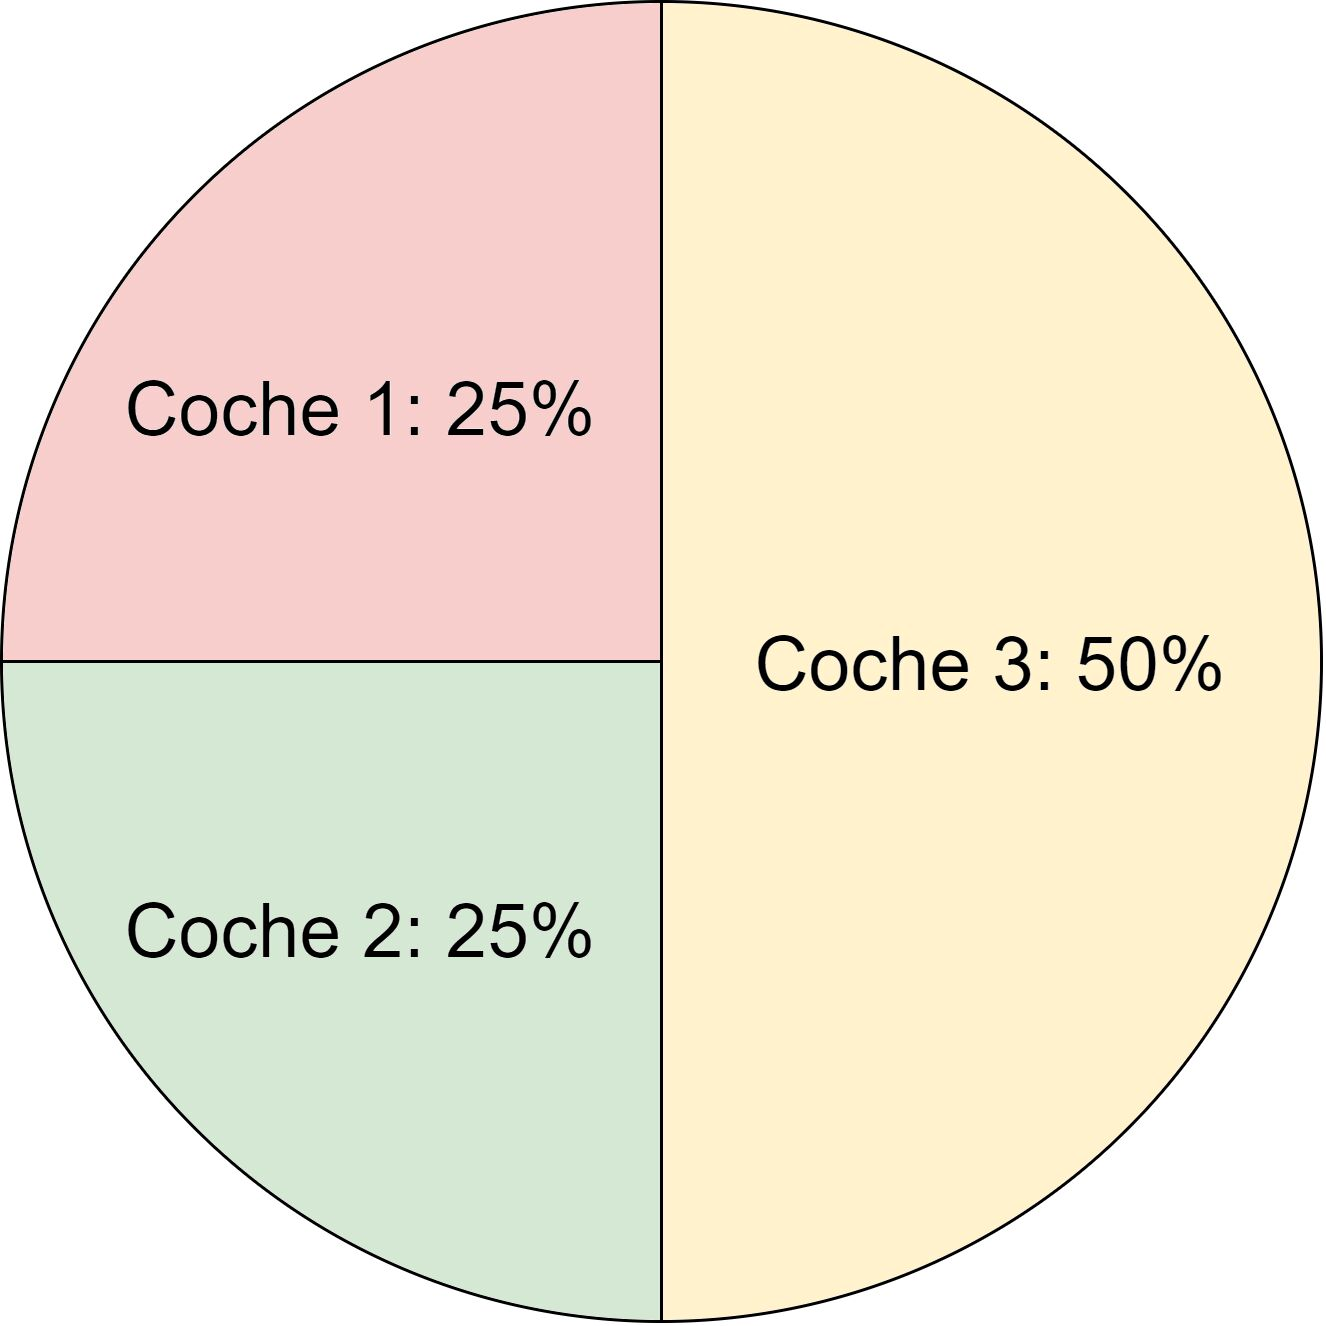
\includegraphics[width=0.4\textwidth]{imagenes/converted/ruleta.jpg}
    \caption{Ilustración de la selección por ruleta}
    \label{fig:ruleta}
\end{figure}

La selección se realiza lanzando una ruleta\cite{gaperformance}, cuyos sectores son divididos en función de la probabilidad calculada anteriormente. La ruleta se debe lanzar tantas veces como padres se desea tener. Una vez que se han elegido los coches que van a ser padres, se emparejan y se mezclan sus constantes para obtener dos hijos de cada pareja. Después, una de las tres constantes del PID en algunos de los hijos puede ser mutada, con una probabilidad del 33\%, con un valor aleatorio de rango [-0.1,0.1] que se le añade al valor existente. Finalmente se sustituyen los coches no elegidos para la siguiente generación por los hijos con las constantes mezcladas y mutadas, manteniendo a los padres, y se vuelve a ejecutar de nuevo el algoritmo.

\bigskip

Utilizando este algoritmo, obtuve unos valores que funcionaban bien para el circuito. No obstante, tras ejecutarlo varias veces, me he dado cuenta de que la constante integral siempre tiende a 0. Para solucionarlo, he decidido obligarle a que tenga un valor mínimo de 0,01.

\newpage

\subsection{Algoritmo de navegación}

En cuanto al algoritmo de navegación, correspondiente a HU2, HU4 y HU5 e implementadas en los sprints 5 y 6, he utilizado A*\cite{4082128}, que es lanzado utilizando diversas reglas, y una componente reactiva. 

\bigskip

A* es utilizado para obtener rutas en un grafo. Para ello, hace uso de una función heurística para estimar la distancia restante al nodo destino. A diferencia de otros algoritmos, como el de Dijkstra, A* es más rápido, gracias a la heurística, ya que puede descartar nodos que están más alejados del destino.

\bigskip

El algoritmo se encarga de visitar todos los nodos vecinos, calculando el coste de llegar desde el origen y el coste para llegar al destino mediante la heurística, en caso de encontrar una ruta mejor de un nodo ya existente en la lista de abiertos, se elimina el anterior y se introduce el nuevo. Este proceso se repite hasta que se llega al destino o, en mi caso, llega a un límite de iteraciones.

\bigskip

Dado que la implementación convencional de A*, haciendo uso de una lista de abiertos para los nodos por visitar y otra de cerrados para los nodos ya visitados, me daba muchos problemas de rendimiento. He decidido mejorarlo eliminando la lista de cerrados y la comprobación de la existencia de una ruta mejor para un nodo que ya se encuentre en la lista de abiertos\cite{a-star}. Esta modificación tiene como desventaja que un mismo nodo puede estar varias veces en la lista de abiertos, pero suele dar mejores resultados\cite{Chen2007PriorityQA}.

\bigskip

Otra mejora ha sido la de utilizar una cola con prioridad para la lista de abiertos, de manera que siempre se encuentre al final (el primero para salir) aquel con menor coste.

\bigskip

Gracias a la cola con prioridad, la desventaja de la nueva versión de A* puede ser solucionada, al priorizarse la ruta más eficiente.


% PONER EJEMPLOS DE RUTAS GENERADAS
\begin{figure}[H]
    \centering
    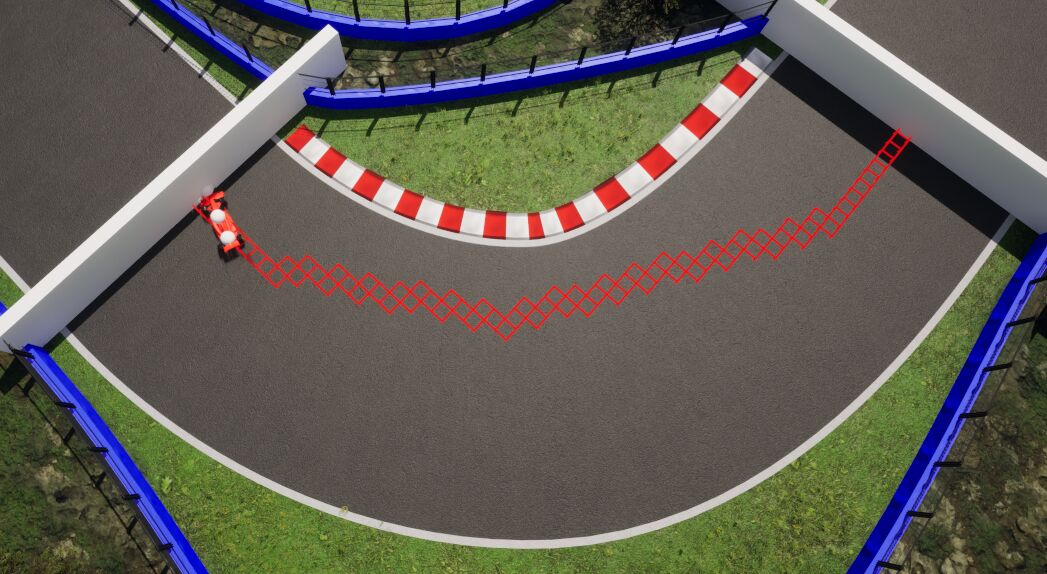
\includegraphics[width=0.7\textwidth]{imagenes/converted/rutaAStar.jpg}
    \caption{Ruta generada por un vehículo hasta el siguiente checkpoint.}
    \label{fig:rutaastar}
\end{figure}


\subsubsection{Heurística}

% Debido a que un nodo puede moverse en 8 direcciones distintas, incluyendo las diagonales, es necesario utilizar una heurística acorde. Por tanto, he decidido utilizar la distancia Chebyshev\cite{enwiki:1149051498}, cuyos movimientos diagonales tienen el mismo coste que los demás. 

% \bigskip

% La configuración de los nodos prohíbe utilizar una heurística como la distancia Manhattan, ya que sobrestimaría la distancia al destino, haciendo que no sea correcto.

La heurística elegida ha sido la distancia Manhattan, ya que el rango de movimiento en la malla es solamente vertical y horizontal.

% foto diagrama de la distancia manhattan
\begin{figure}[H]
    \centering
    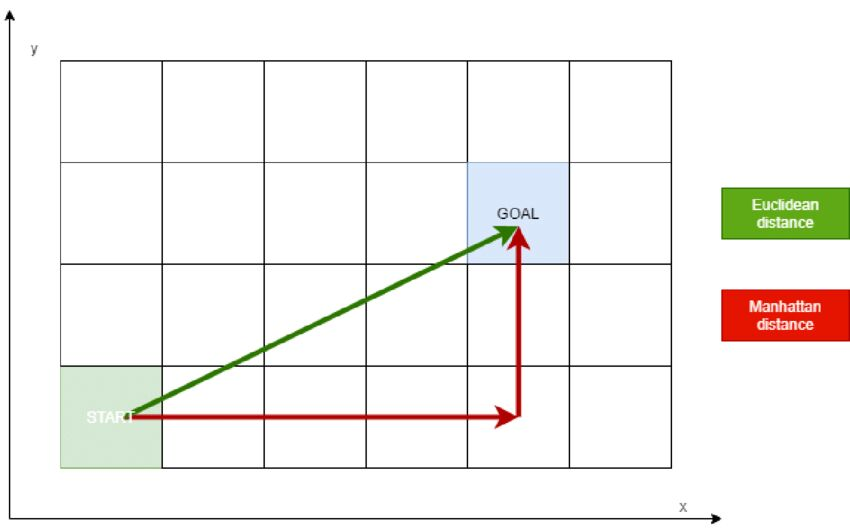
\includegraphics[width=0.7\textwidth]{imagenes/converted/Euclidean-and-Manhattan-distance-comparison-3235-Optimizations-The-first-optimization.jpg}
    \caption{Esquema del funcionamiento de la distancia Manhattan\cite{gameai}.}
    \label{fig:manhattan}
\end{figure}


\subsection{Generación de la malla de navegación}
Para que A* funcione, es necesario discretizar el espacio y crear una estructura de datos que permita incluir todos los posibles estados para que los pilotos puedan tomar decisiones.

\bigskip

% En cada subsección se hablará de cada componente que forma la malla de navegación:
A continuación se da una explicación de cada uno de los elementos que forman la malla de navegación:

\begin{itemize}
    \item \textbf{Nodo: }Para implementarlo, he creado un actor (véase sección \ref{sec:terminosunreal}) que representa un nodo. Además, posee las variables necesarias para saber si se encuentra un vehículo dentro de él, si es un delimitador de límites de pista, si es un checkpoint o si es una guía de ruta óptima. De esta forma se puede tener un control muy alto sobre los pesos de cada estado.
    
    \bigskip
    
    La actualización de un nodo de un estado a otro se realiza mediante el evento \textit{ActorBeginOverlap} y \textit{ActorEndOverlap} (véase sección \ref{sec:terminosunreal}). Así se puede actualizar el mapa en tiempo real.
    
    \bigskip
    
    Cabe destacar que los nodos con estado checkpoint y delimitador no pueden ser cambiados de estado; es decir, el delimitador de pista siempre estará ocupado, dándole un coste mayor. Mientras que el checkpoint siempre estará libre, dándole un coste menor. Los checkpoints nunca reciben colisión para optimizar la velocidad del algoritmo A*, ya que si se tienen en cuenta puede llegar a tardar demasiado en encontrar la ruta.
    
    \bigskip
    
    El estado ruta óptima sirve para darle una ayuda a los coches, ya que si no se utilizase escogería rutas más rígidas. Este estado no prohíbe a los coches la posibilidad de elegir otra ruta para adelantar o volver a pista, solo es una guía.
    
    \bigskip
    
    La construcción del delimitador y de la ruta óptima la he realizado utilizando actores distintos, de manera que se activen los eventos anteriormente mencionados para que se ajusten.
    
    \bigskip
    
    Por último, cada nodo también almacena una referencia a sus nodos adyacentes, para que puedan ser utilizados por el algoritmo A*.

    \begin{figure}[H]
        \centering
        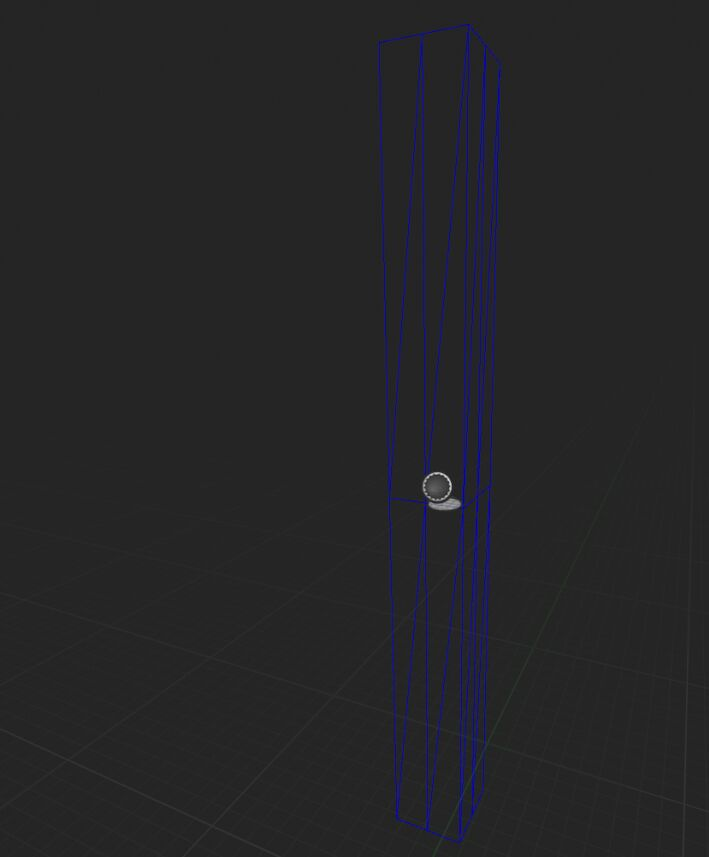
\includegraphics[width=0.5\textwidth]{imagenes/converted/nodo.jpg}
        \caption{Representación de un nodo en Unreal Engine.}
        \label{fig:nodo}
    \end{figure}

    \item \textbf{Malla (conjunto de nodos): }Para realizar la malla de navegación he utilizado un actor encargado de generar los nodos mencionados anteriormente en una malla de \gridSize. Como he dicho antes, estos valores pueden ser modificados, incluido el offset de donde comienza a generar nodos.
    
    \bigskip
    
    Este actor incluye los métodos necesarios para poder direccionar un nodo de la malla como una matriz (con filas y columnas), poder obtener su posición en coordenadas del mundo y poder convertir de coordenadas del mundo a coordenadas de matriz.

    % foto de la malla recreada en unreal
    \begin{figure}[H]
        \centering
        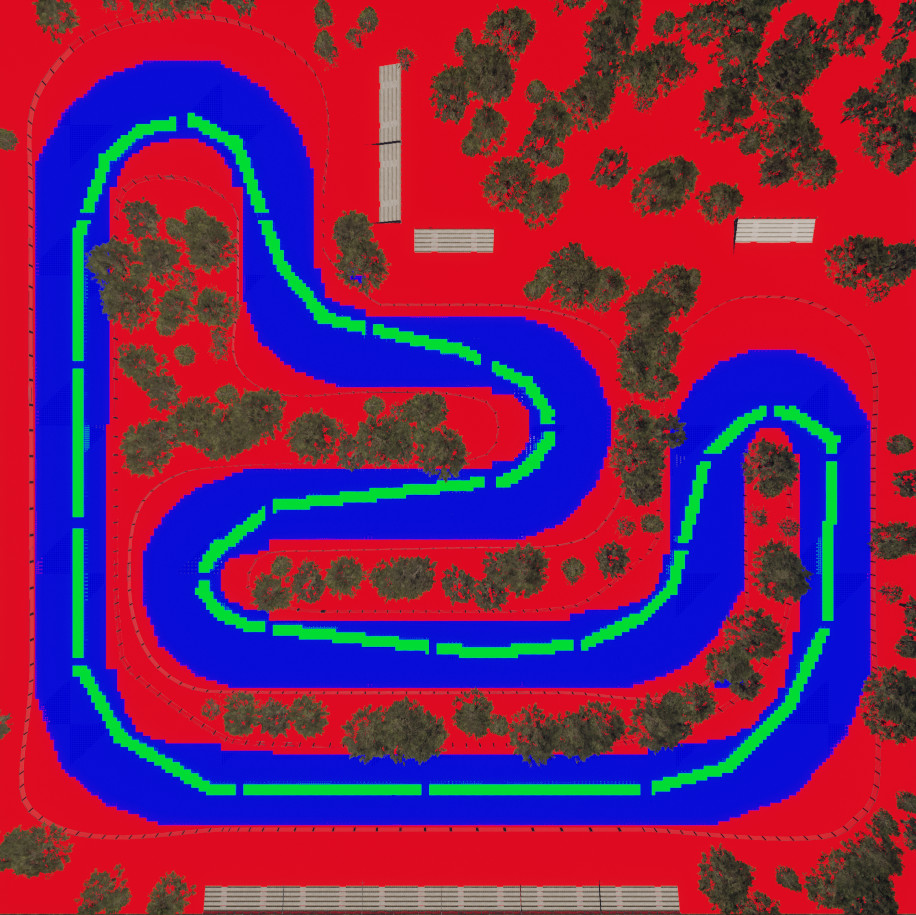
\includegraphics[width=0.6\textwidth]{imagenes/converted/malla.jpg}
        \caption{Malla de navegación generada sobre el circuito. Los puntos rojos son muros, los verdes indicadores de ruta óptima y los azules el resto de la pista usable.}
        \label{fig:mallanav}
    \end{figure}
\end{itemize}
% \subsubsection{Nodo}
% \subsubsection{Malla de navegación}

\newpage

\subsection{Cálculo de la ruta por los vehículos}

Con todo lo anterior implementado el coche es capaz de obtener una ruta por el circuito. No obstante, sigue siendo demasiado costoso obtener una ruta demasiado larga, para luego tener que desecharla por un adelantamiento o un choque. Es por eso que he dividido el circuito en varios checkpoints de tamaño relativamente reducido, con el objetivo de que el cálculo de rutas sea más rápido.


% foto de los checkpoints
\begin{figure}[H]
    \centering
    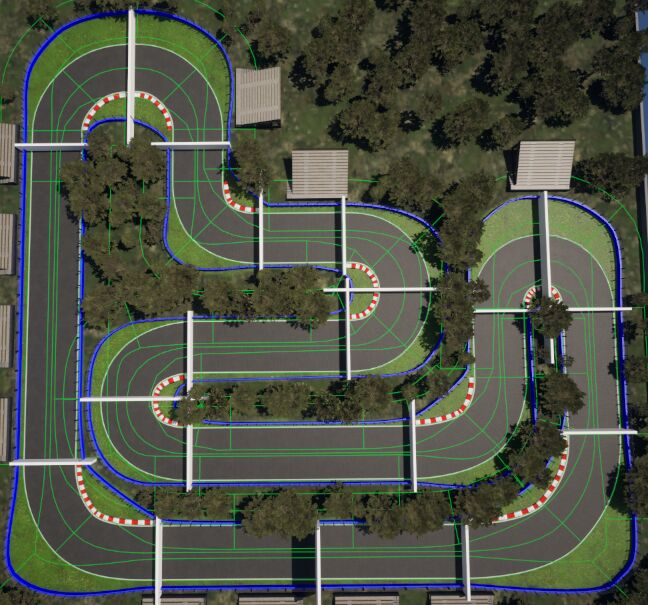
\includegraphics[width=0.6\textwidth]{imagenes/converted/checkpoints.jpg}
    \caption{Checkpoints utilizados a lo largo del circuito. Los checkpoints son las barreras de color blanco.}
    \label{fig:checkpointunreal}
\end{figure}

Cuando la parte delantera del vehículo se solapa con un checkpoint, calcula la ruta utilizando A* hasta el siguiente. La llamada al algoritmo devuelve un vector de puntos en coordenadas del mundo. El vehículo se encarga de filtrar los puntos generados para que solo haya uno en cada checkpoint, ya que en otro caso puede generar problemas en el seguimiento de la ruta.

\bigskip

Con los puntos filtrados, el coche construye un spline y pinta los puntos en el suelo. Este spline será seguido gracias al controlador PID (Figura \ref{fig:pidbp}) mencionado anteriormente. Cabe destacar que al ser la ruta discreta y el vehículo una componente física del mundo, el vehículo no siempre conseguirá seguirla siempre, pero le servirá como ``guía'' a la hora de tener que hacer giros y adelantamientos.

\newpage

\subsection{Lógica de adelantamiento de los vehículos}

Dado que el algoritmo A* funciona principalmente para mundos estáticos, es necesario actualizar la ruta si se realiza un cambio de posición en los vehículos. En este caso, para adelantar al contrincante.

\bigskip

La regla que sigue el vehículo es si se encuentra a una distancia del vehículo de adelante y tiene la suficiente diferencia de velocidad, ejecuta el algoritmo de navegación y espera unos pocos segundos para volverlo a ejecutar. Esta implementación me ha dado unos resultados razonables en tiempo y habilidad en los pilotos.

% quizas poner foto, pero creo que va a ser complicado
\begin{figure}[H]
    \centering
    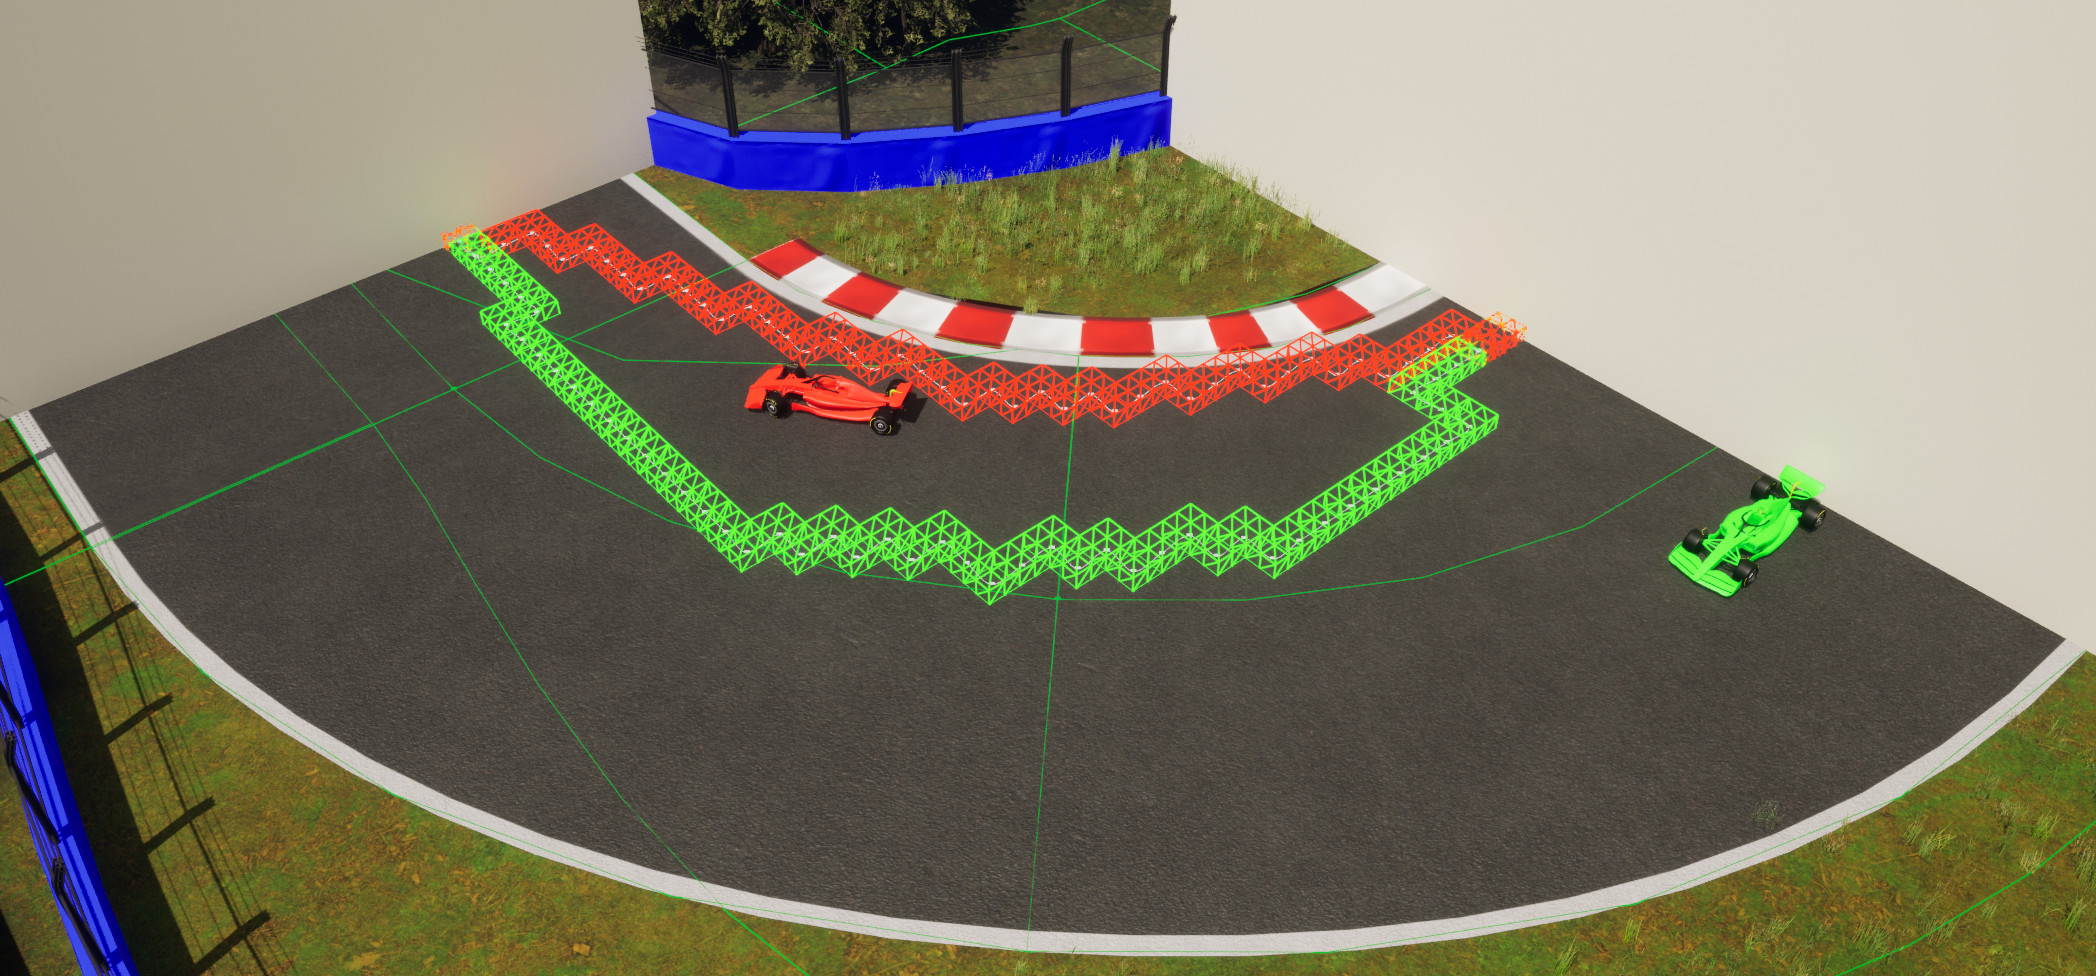
\includegraphics[width=0.6\textwidth]{imagenes/converted/overtake.jpg}
    \caption{Cálculo de la ruta del coche verde para intentar adelantar al otro piloto.}
    \label{fig:overtake}
\end{figure}

\subsection{Recuperación después de un accidente}

Si un coche se sale de pista primero se esperan unos segundos para comprobar que de verdad no se puede mover. Cuando se ha comprobado, se recorre un cierto tiempo marcha atrás con las ruedas rectas. Finalmente, ejecuta el A* para calcular una ruta de escapatoria y recorre lento dicha ruta por un breve instante de tiempo, hasta que finalmente recupera la velocidad que tenía.

\subsection{Recuperación después del vuelco}

Puede darse el remoto caso de que un vehículo vuelque y no sea capaz de darse la vuelta. En este caso he decidido implementar una regla que comprueba si la rotación del coche es mayor de 90 grados en ambos sentidos, pone el coche de nuevo sobre sus cuatro ruedas.

\subsection{Control de acelerador y freno}

El control del acelerador y del freno en condiciones normales de carrera se implementa incluyendo en cada checkpoint (Figura \ref{fig:checkpointunreal}) la velocidad recomendada a la que debe ir el coche. El coche calcula la distancia a la que se encuentra del siguiente checkpoint y la distancia de frenado necesaria basándose en la velocidad y la desaceleración por el frenado (también se incluye la componente de agresividad, que se explicará más tarde).

\bigskip

Cabe destacar que esta velocidad es modificada por el estado del piloto, que se explicará en secciones posteriores.

\subsection{Algoritmo para las posiciones de los pilotos}

En lo que se refiere al cálculo de las posiciones de cada piloto, correspondientes a HU7 y HU8 e implementadas en el sprint 7, he utilizado una estructura de datos algo más compleja. Los vehículos almacenan la vuelta en la que están y el checkpoint; es decir, el sector del circuito en el que se encuentran. Con la información anterior, he creado un array asociativo que almacene como clave la vuelta y como valor otro array asociativo, que a su vez tiene como clave el checkpoint y como valor un array con todos los vehículos que se encuentran en ese estado. Para mostrarlo, solo hace falta iterar primero por aquellas claves mayores, ya que son los que más vueltas y más lejos del circuito están.

\begin{table}[H]
    \centering
    \begin{tblr}{
        cells = {c},
        row{1} = {Silver},
        cell{1}{2} = {c=2}{},
        cell{2}{1} = {r=4}{},
        cell{2}{2} = {Alto},
        cell{2}{3} = {Alto},
        cell{7}{1} = {r=2}{},
        cell{7}{2} = {Alto},
        cell{7}{3} = {Alto},
        vlines,
        hline{1-2,6-7,9} = {-}{},
        hline{3-5,8} = {2-3}{},
            }
        \textbf{Clave (vuelta actual)} & \textbf{Valor }                    &                \\
        0                              & \textbf{Clave (checkpoint actual)} & \textbf{Valor} \\
                                       & 0                                  & {[}c1]         \\
                                       & ...                                &                \\
                                       & i                                  & {[}c2, c3]     \\
        ...                            & ...                                & ...            \\
        i                              & \textbf{Clave (checkpoint actual)} & \textbf{Valor} \\
                                       & 3                                  & {[}c4]
    \end{tblr}
    \caption{Representación de la estructura de datos que almacena las posiciones de los pilotos durante la carrera.}
    \label{fig:tablapos}
\end{table}

% Para saber cuando lanzar la actualización de la lista de posiciones, cada coche calcula si el que está por delante de él sigue así, en caso contrario lanza el evento de actualización.

Para saber cuando lanzar la actualización de la lista de posiciones, cada coche comprueba si ha conseguido adelantar al coche que estaba inmediatamente delante de él, en caso afirmativo lanza el evento de actualización.


\subsection{Contador de vueltas}

En cuanto a la actualización del contador de vueltas, correspondiente a HU9 y realizado en el sprint 8, he hecho que todos los coches cuando acaben una vuelta intenten actualizarlo, en caso de que la vuelta actual sea mayor o igual, no se actualiza. De esta forma, es más fácil llevar un control más preciso de las vueltas.


\section{Modelado y texturizado de la escena}

Para la creación, preparación y modificación de los distintos modelos y texturas de la aplicación, he utilizado Blender\cite{blender} y GIMP\cite{gimp}. A continuación detallaré cada uno de los modelos y texturas, así como su proceso de creación.

\subsection{Trazado del circuito}

El trazado de la carretera lo he realizado creando primero un spline en Unreal con la forma deseada. A continuación, se debe incluir un modelo de carretera para que el spline pueda generarlo siguiendo la forma del trazado.
\begin{figure}[H]
    \centering
    % \includegraphics[width=\textwidth]{imagenes/converted/trazado.jpg}
    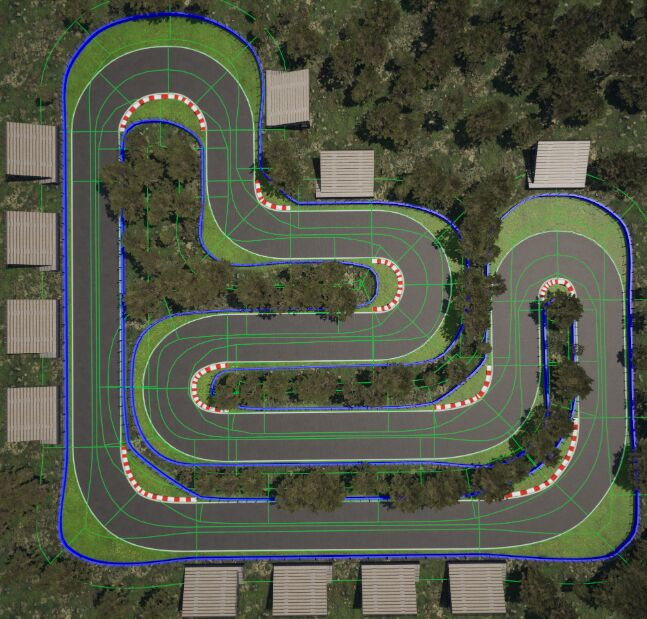
\includegraphics[width=0.7\textwidth]{imagenes/converted/trazadoFinal.jpg}
    \caption{Trazado del circuito final.}
    \label{fig:trazado}
\end{figure}


En la vida real, los circuitos suelen tener secciones donde la carretera es recta y otras secciones donde se incluyen pianos, especialmente en las curvas. Por lo tanto, ha sido necesario crear tres modelos distintos de pista: uno sin piano, otro con piano a la izquierda y otro con el piano a la derecha. De esta manera, se logra una representación más fiel y realista de las diferentes secciones del circuito.

\bigskip

He utilizado Blender para generar los tres modelos de pista. Las secciones se construyeron a partir de un cubo achatado, y en las versiones con piano, se ha extruido uno de los lados y se ha aplicado un \textit{bevel} para suavizar las esquinas.

% fotos de las 3 versiones
\begin{figure}[H]
    \centering
    \begin{subfigure}[t]{0.48\textwidth}
        \centering
        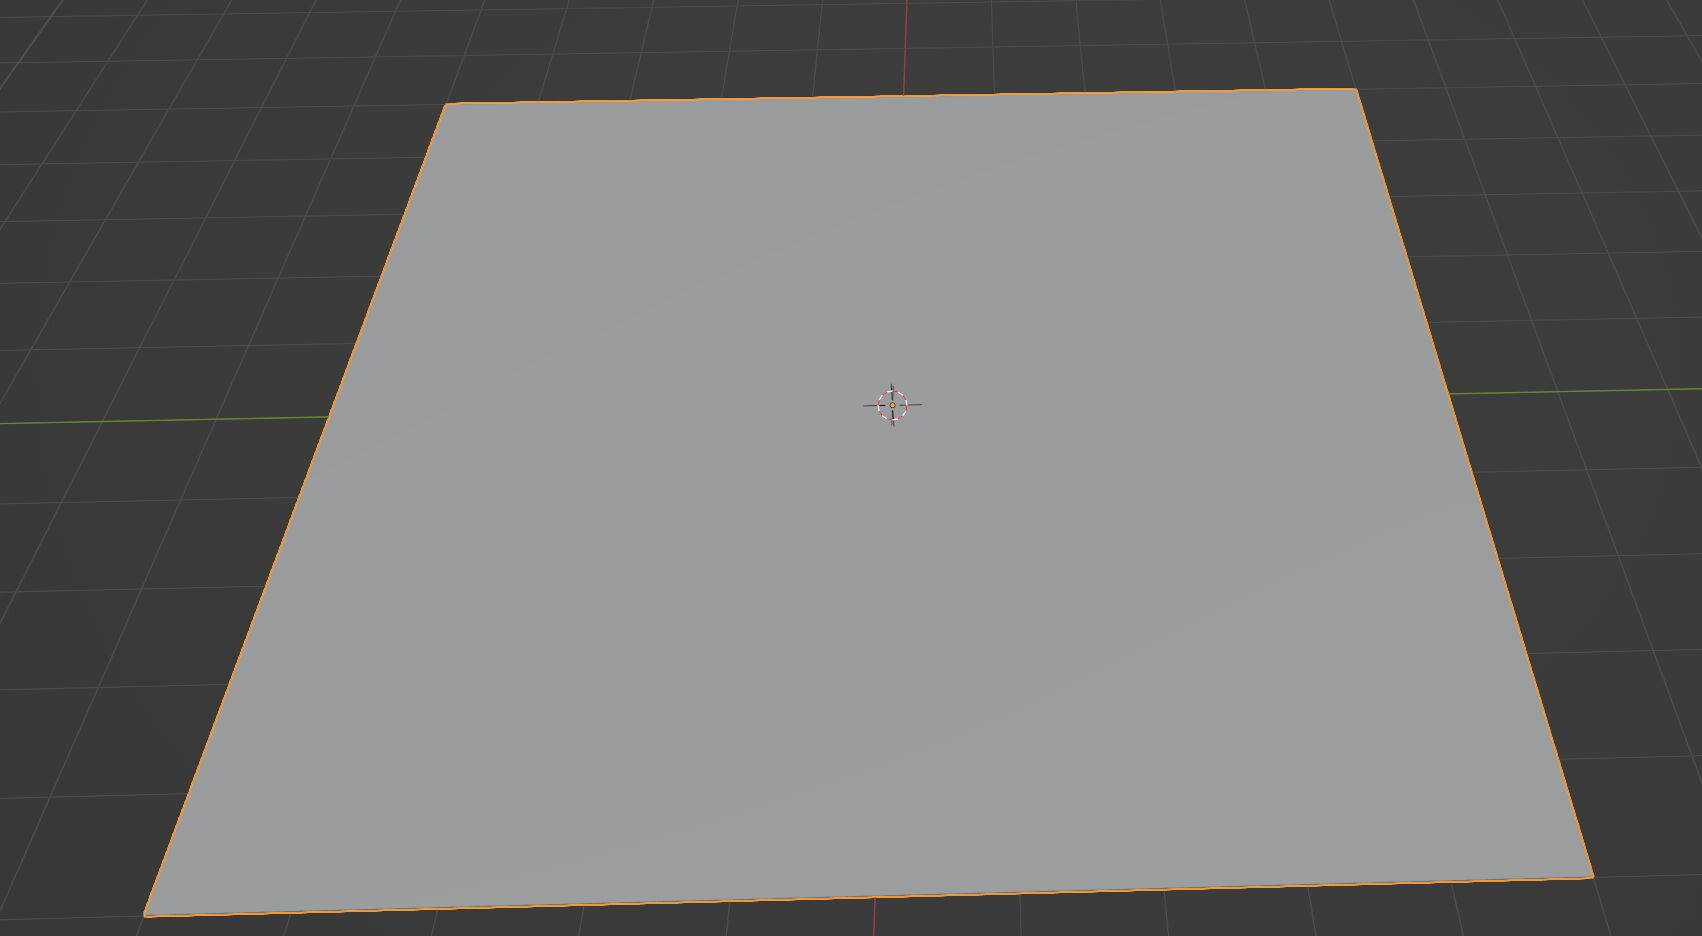
\includegraphics[width=\textwidth]{imagenes/converted/pista/curva-recta.jpg}
        \caption{Sección recta de la curva.}
        \label{fig:curvarecta}
    \end{subfigure}
    \hfill
    \begin{subfigure}[t]{0.48\textwidth}
        \centering
        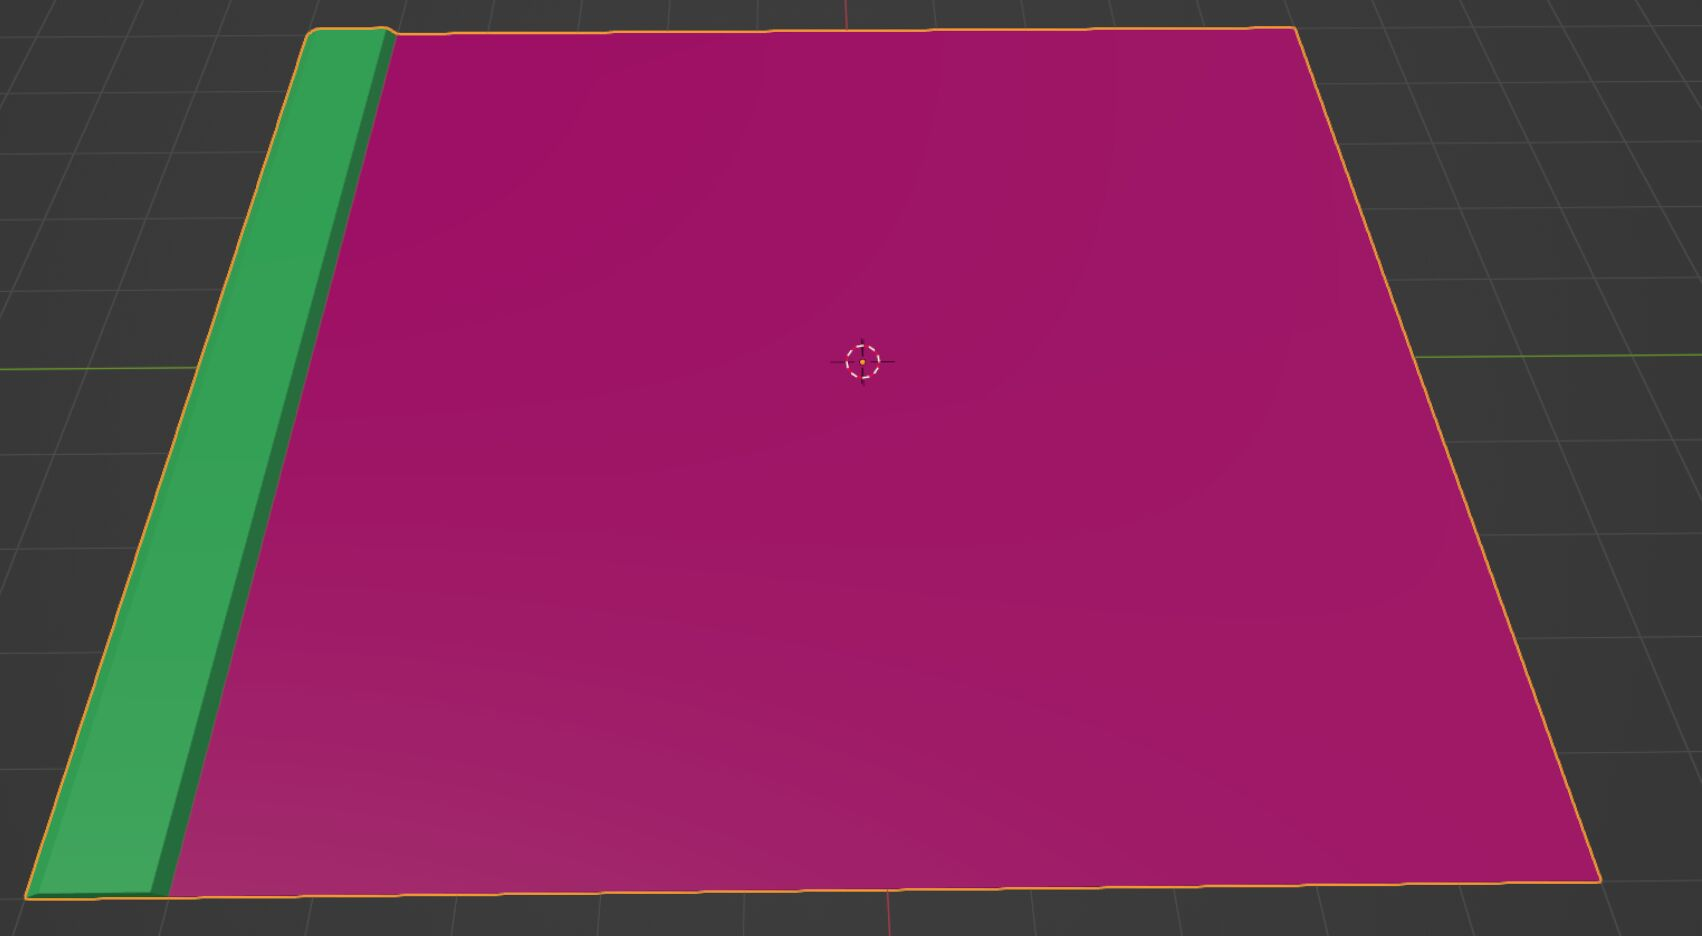
\includegraphics[width=\textwidth]{imagenes/converted/pista/curva.jpg}
        \caption{Sección con el piano a la izquierda.}
        \label{fig:curvaL}
    \end{subfigure}
    \par\bigskip
    \begin{subfigure}[t]{0.48\textwidth}
        \centering
        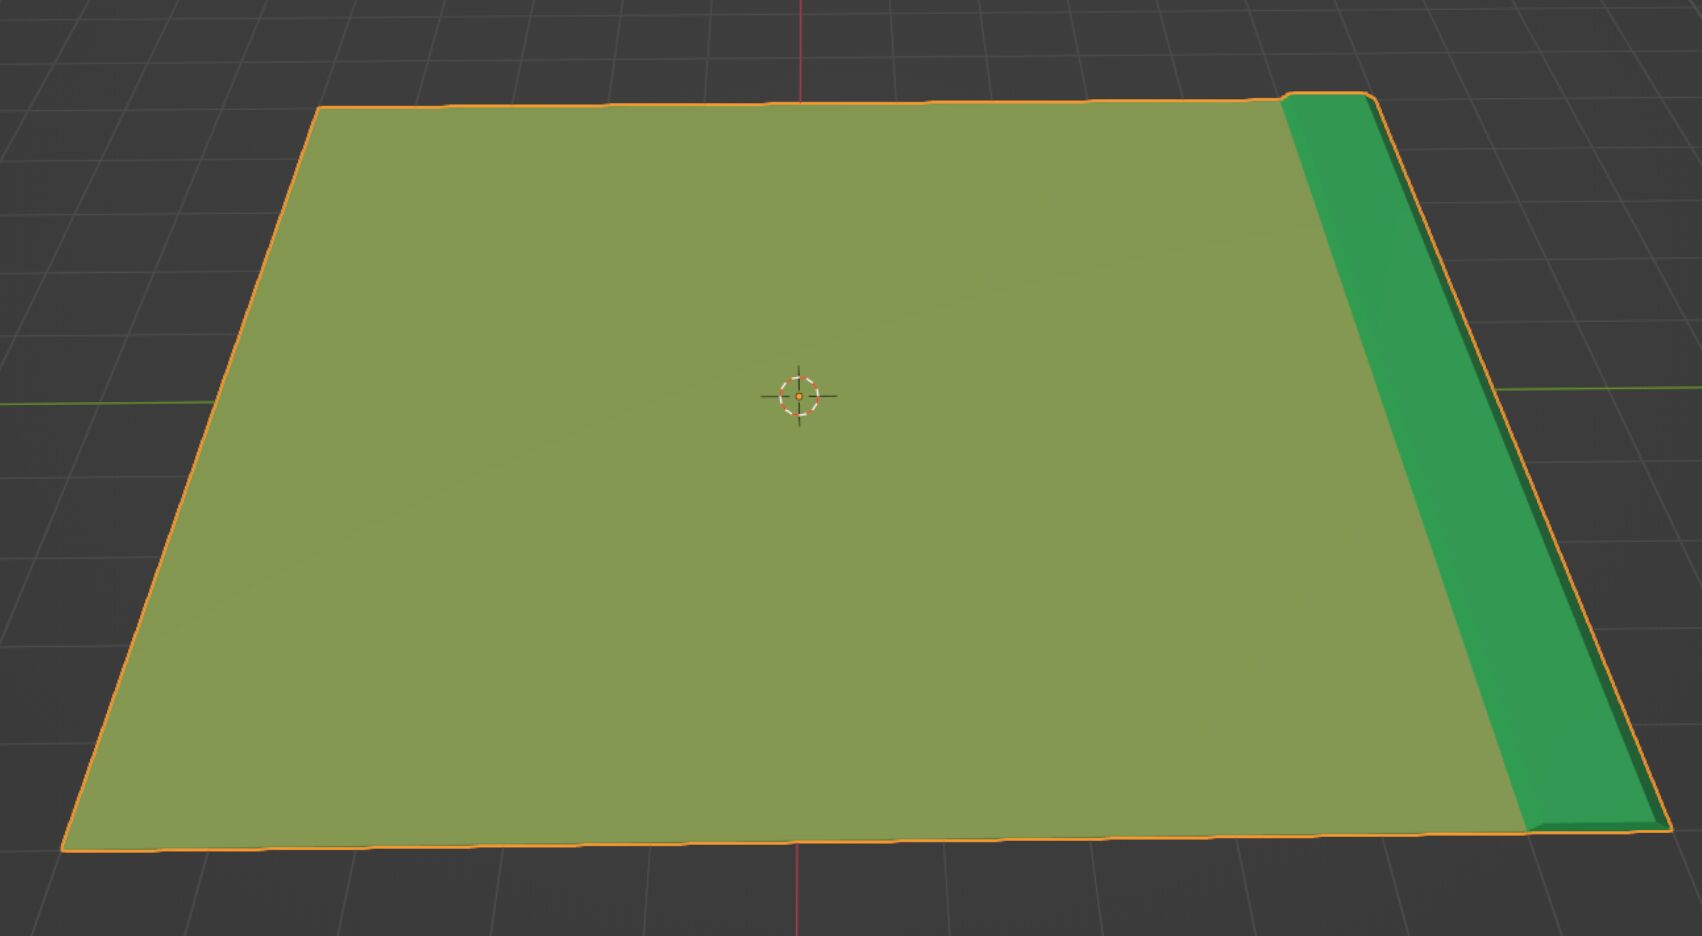
\includegraphics[width=\textwidth]{imagenes/converted/pista/curva-inverted.jpg}
        \caption{Sección con el piano a la derecha.}
        \label{fig:curvaR}
    \end{subfigure}
    \caption{Modelos de pista utilizados.}
    \label{fig:curvasmodelos}
\end{figure}

Después, he utilizado la textura ``Asphalt 024 A''\cite{asphalt}, creada por Lennart Demes, y he modificado la componente difusa utilizando GIMP para poner una línea continua a ambos extremos, similar a los circuitos reales.

\begin{figure}[H]
    \centering
    
\includegraphics[width=0.4\textwidth,cframe=black 0.5pt 0pt]{imagenes/converted/pista/Asphalt024A_2K_Color.jpg}
    \caption{Textura de asfalto modificada. Enmarcado para diferenciar con el color de la página.}
    \label{fig:asfaltomod}
\end{figure}

Para texturizar el piano, he decidido crear la textura yo. Utilizando GIMP, he creado una textura difusa con un tamaño de 2048x2048 píxeles y he pintado una mitad de color blanco y la otra de color rojo. 


\begin{figure}[H]
    \centering
    
\includegraphics[width=0.4\textwidth]{imagenes/converted/pista/kerb-dirty2.jpg}
    \caption{Textura utilizada para la componente difusa del piano.}
    \label{fig:pianodiff}
\end{figure}

El resultado en Unreal no era del todo convincente, ya que los bordes tenían demasiada iluminación. Para solucionarlo, he creado una textura para la componente de oclusión ambiental, de forma que los bordes sean algo más oscuros que la parte central. 

\begin{figure}[H]
    \centering
    
\includegraphics[width=0.4\textwidth,cframe=black 0.5pt 0pt]{imagenes/converted/pista/kerb-dirty2-AO.jpg}
    \caption{Textura utilizada para la oclusión ambiental del piano. Enmarcado para diferenciar del fondo de la página.}
    \label{fig:pianoao}
\end{figure}

Estas texturas no encajaban del todo bien, haciendo que las líneas blancas no estuviesen alineadas con los bordes y que la textura del piano no se repitiese varias veces en la sección. Utilizando Blender, he realizado un mapeado UV de los modelos, con el objetivo de que la asignación de las texturas se realice correctamente.

\begin{figure}[H]
    \centering
    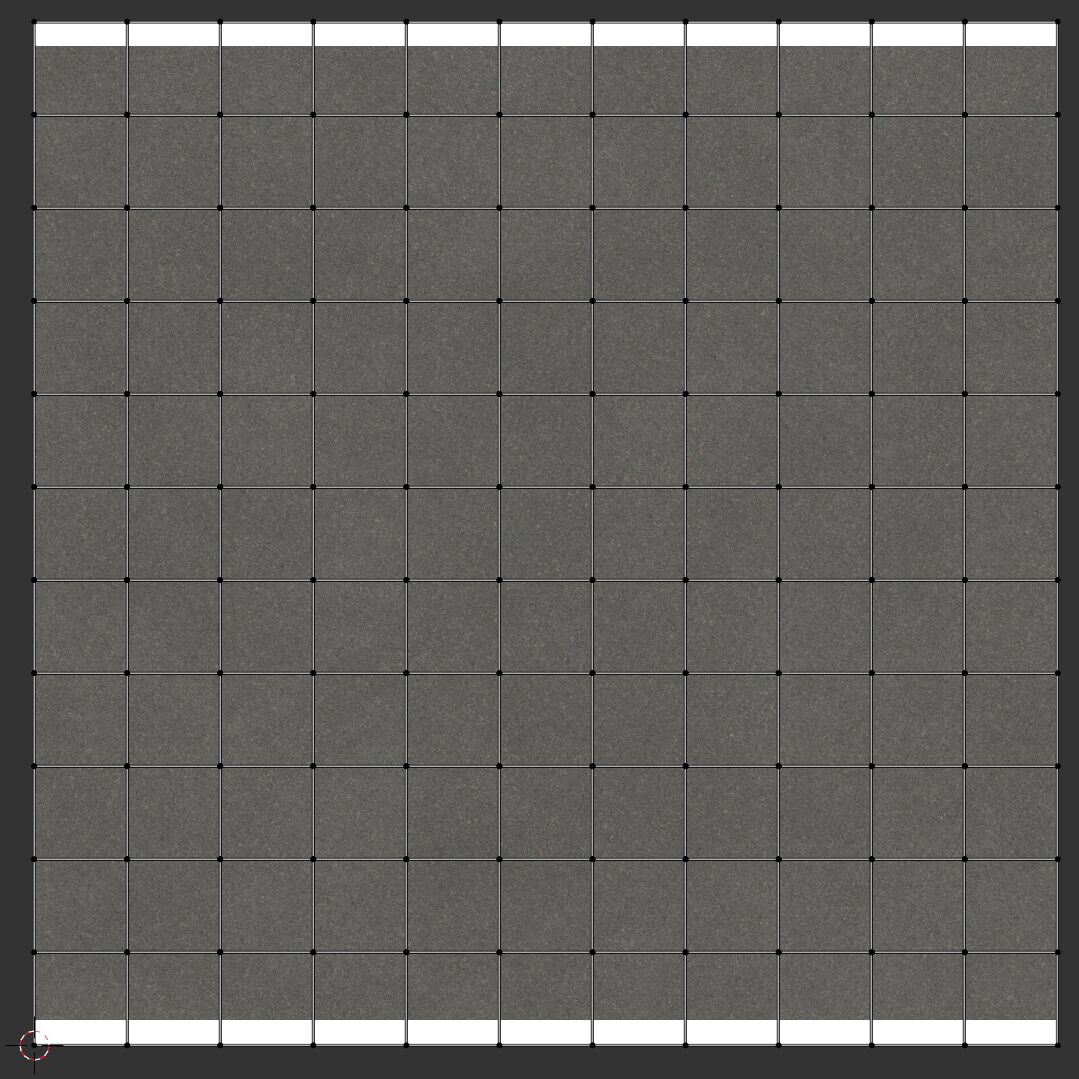
\includegraphics[width=0.4\textwidth]{imagenes/converted/pista/uv-straight.jpg}
    \caption{Mapeado UV para la sección de asfalto.}
    \label{fig:uvasphalt}
\end{figure}

\begin{figure}[H]
    \centering
    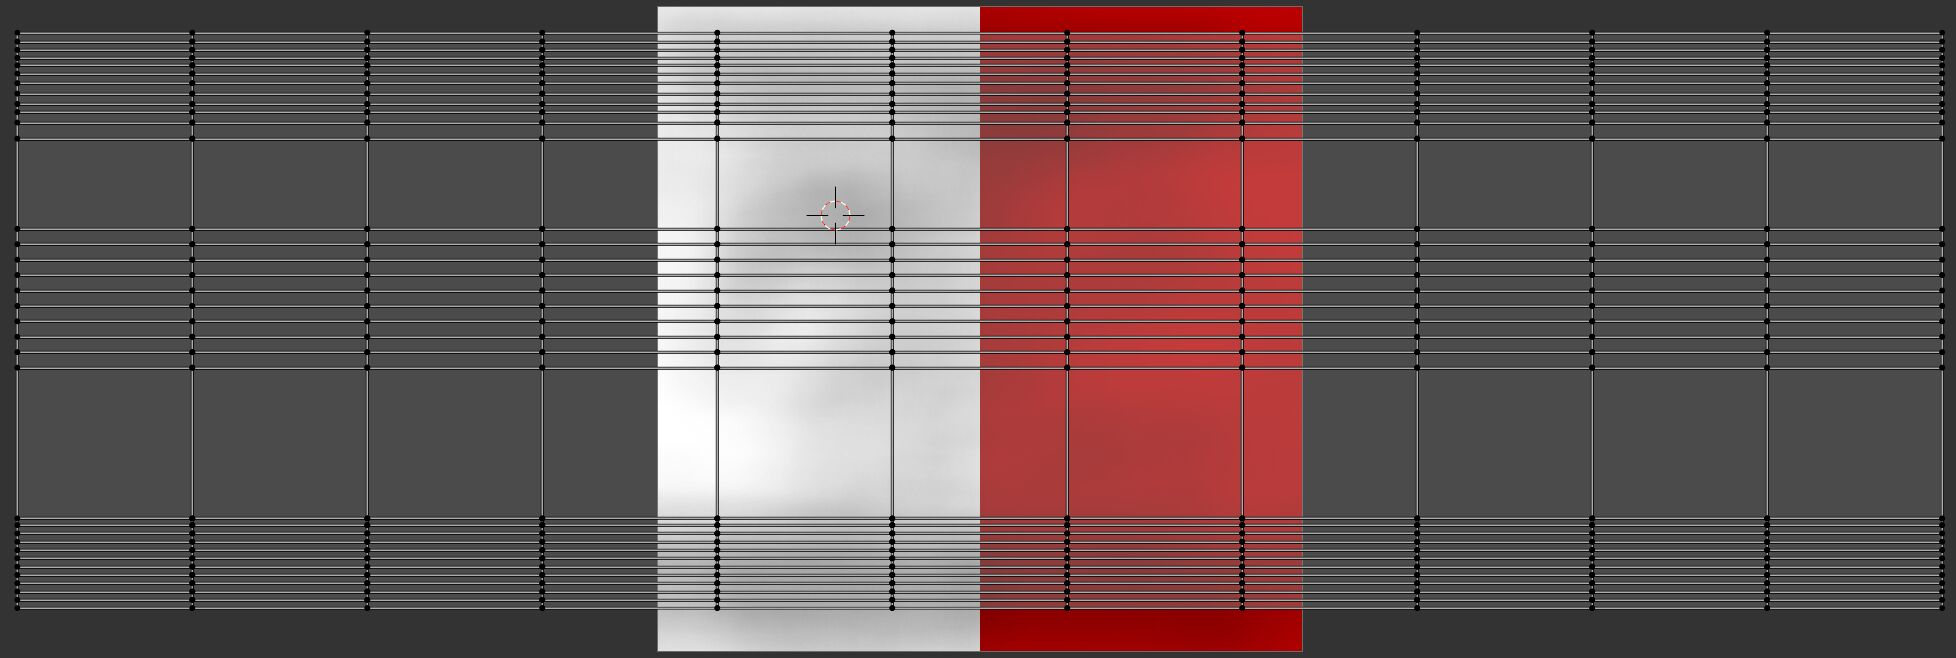
\includegraphics[width=0.8\textwidth]{imagenes/converted/pista/uv-kerb.jpg}
    \caption{Mapeado UV para la sección de piano.}
    \label{fig:uvkerb}
\end{figure}

Ahora sí se sitúan bien las texturas en el modelo. A continuación se encuentran las imágenes del resultado final en Unreal.

\begin{figure}[H]
    \centering
    \begin{subfigure}[t]{0.48\textwidth}
        \centering
        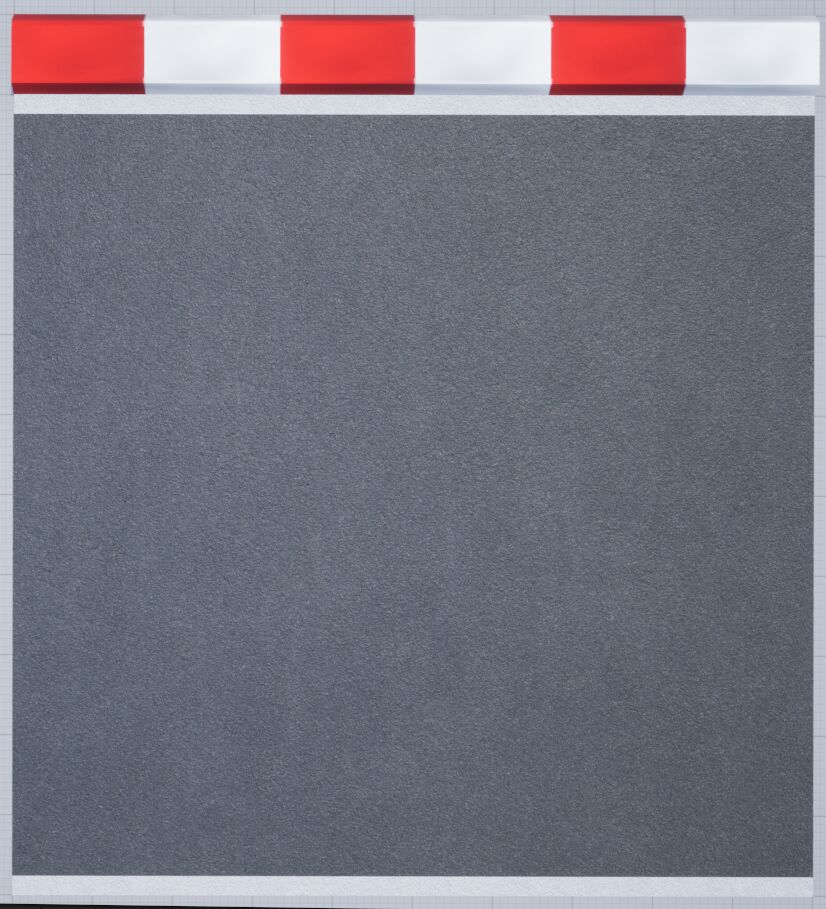
\includegraphics[width=\textwidth]{imagenes/converted/pista/track-final.jpg}
        \caption{Sección de pista con el piano a la derecha.}
        \label{fig:curvafinal2}
    \end{subfigure}
    \hfill
    \begin{subfigure}[t]{0.48\textwidth}
        \centering
        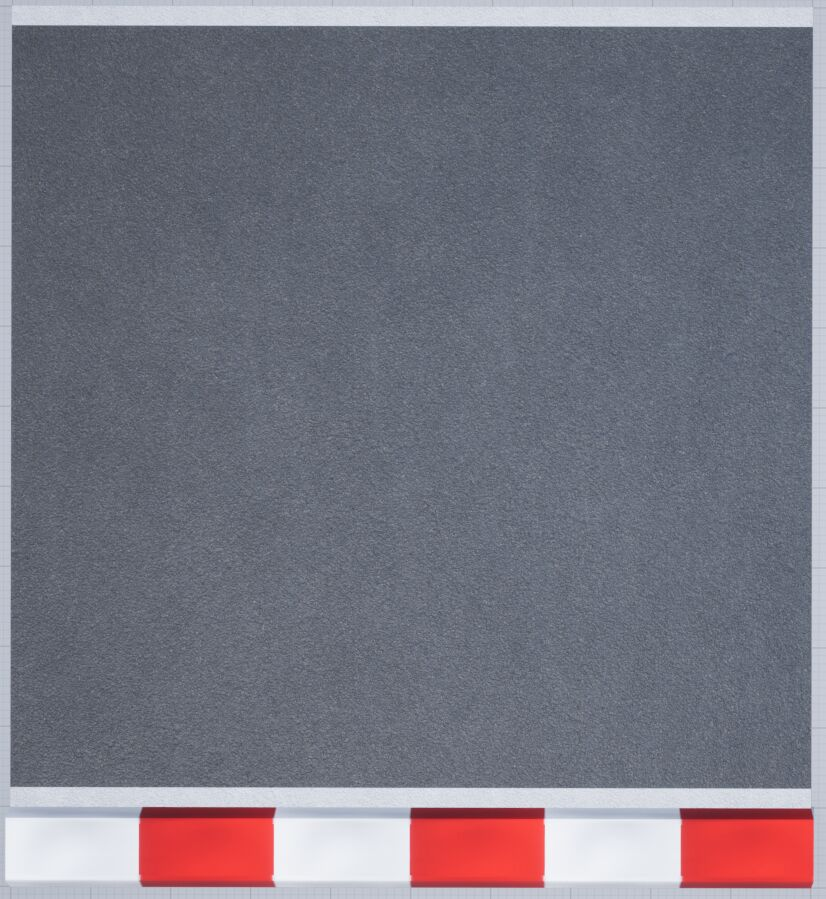
\includegraphics[width=\textwidth]{imagenes/converted/pista/track-final-inverted.jpg}
        \caption{Sección de pista con el piano a la izquierda.}
        \label{fig:curvafinla3}
    \end{subfigure}
    \par\bigskip
    \begin{subfigure}[t]{0.48\textwidth}
        \centering
        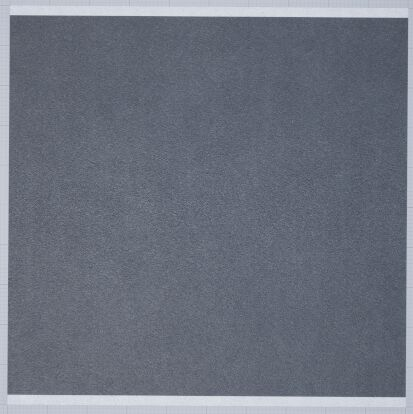
\includegraphics[width=\textwidth]{imagenes/converted/pista/track-straight-final.jpg}
        \caption{Sección de pista recta.}
        \label{fig:curvafinal1}
    \end{subfigure}

    \caption{Secciones de pista finales en Unreal.}
    \label{fig:seccionespista}
\end{figure}

\newpage

\subsection{Preparación de los coches}

Debido a que modelar un vehículo requiere demasiado tiempo, he optado por utilizar el modelo ``Porsche 911 GT3''\cite{porsche} realizado por ``ChevroletSS'' y el modelo ``Mercedes F1 W14''\cite{f1} realizado por ``3dblenderlol''. Además, he eliminado toda clase de logotipos y marcas de los vehículos, para facilitar la exportación.

\bigskip

A continuación, es necesario preparar los modelos para que las ruedas se puedan mover en Unreal. Se debe realizar un \textit{rigging} de las ruedas; es decir, asignarle un conjunto de huesos, que actuarán como ejes para la rotación de las ruedas. Esta tarea la he realizado cargando los modelos y utilizando el plugin de Blender ``UE4 Vehicle Rigging Addon for Blender''\cite{blenderplugin}, creado por ``Continue Break''. El plugin permite realizar el \textit{rigging} de manera automática con tan solo indicarle el chasis del coche y sus ruedas.

\begin{figure}[H]
    \centering
\begin{subfigure}[t]{0.48\textwidth}
    \centering
    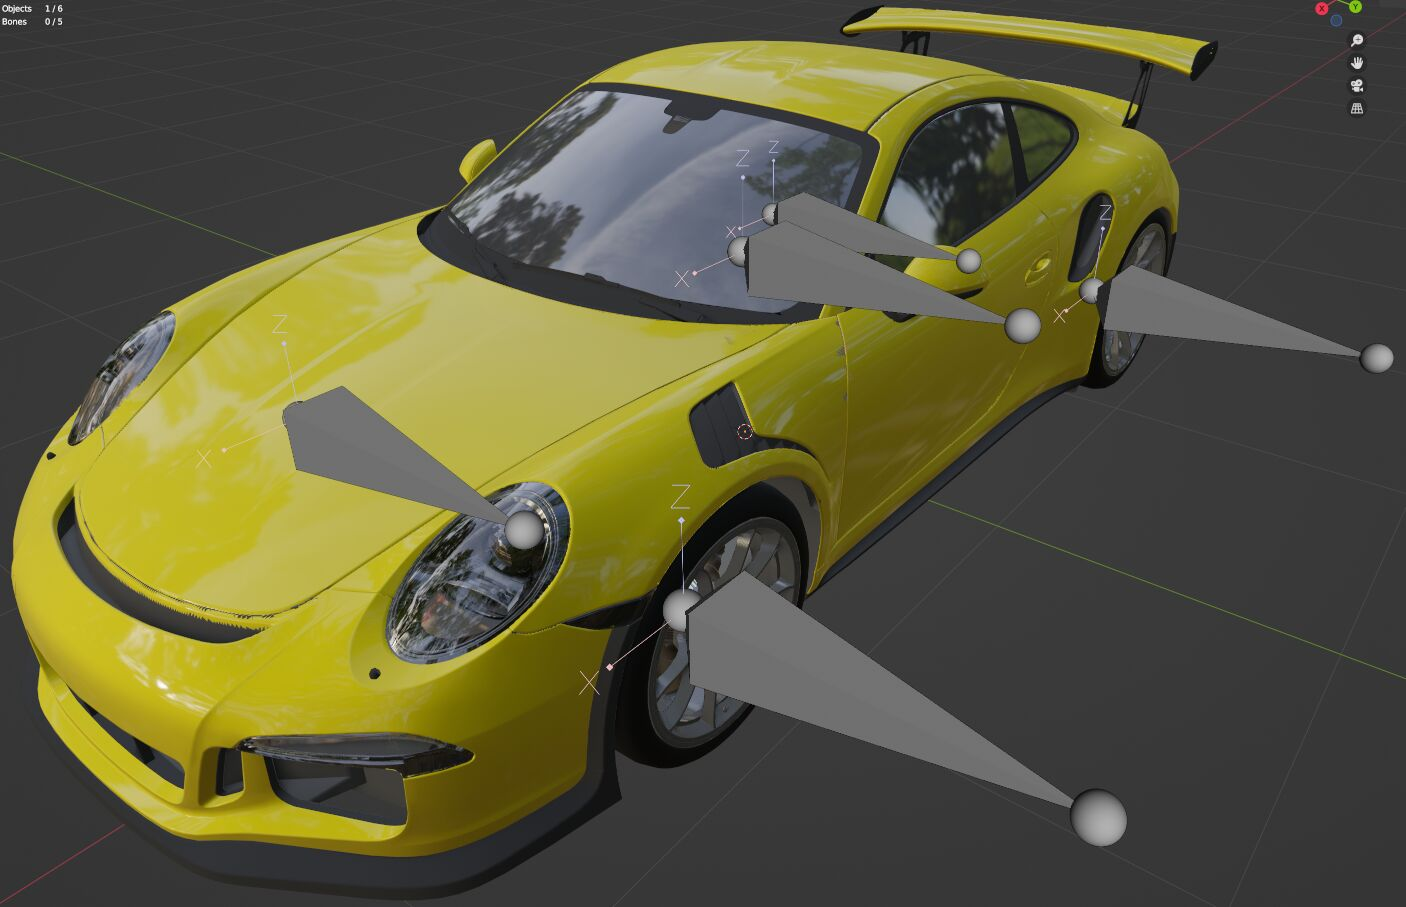
\includegraphics[width=\textwidth]{imagenes/converted/rigging/911-rigging.jpg}
    \caption{\textit{Rigging} realizado en el Porsche 911.}
    \label{fig:rigging911}
\end{subfigure}
\hfill
\begin{subfigure}[t]{0.48\textwidth}
    \centering
    % \includegraphics[width=\textwidth]{imagenes/trazado.jpg}
    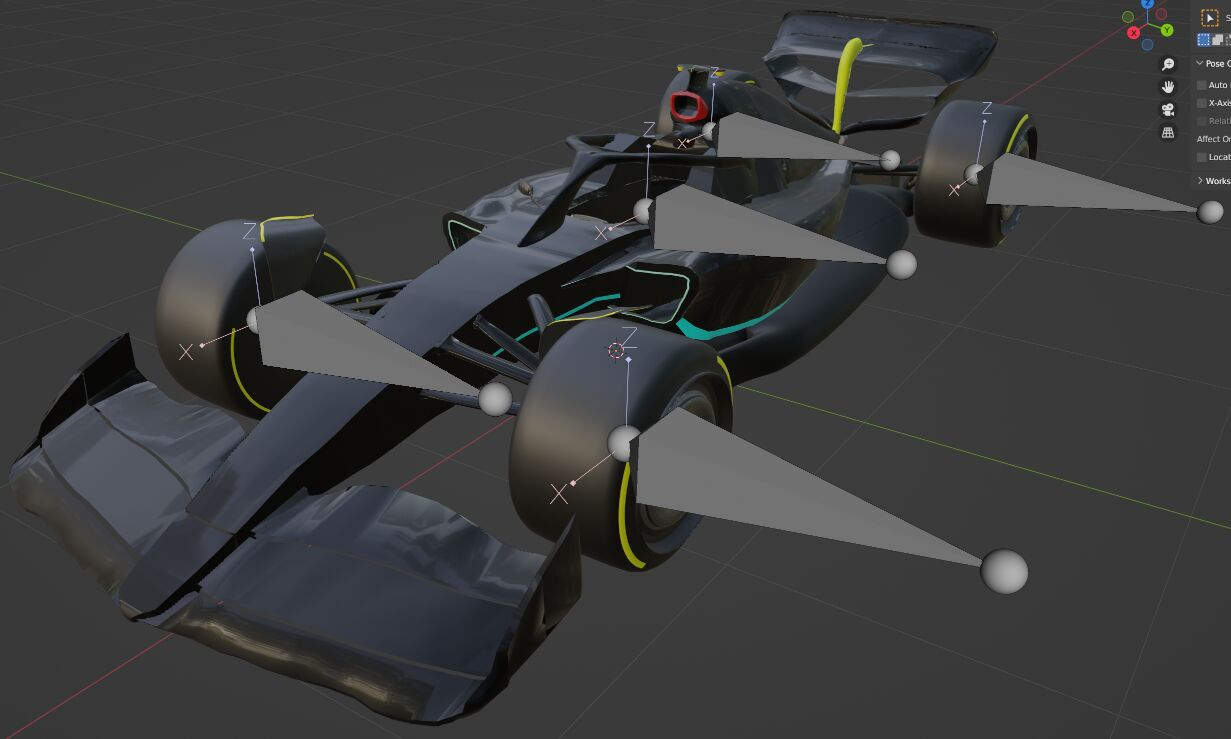
\includegraphics[width=\textwidth]{imagenes/converted/rigging/f1-rigging.jpg}
    \caption{\textit{Rigging} realizado en el coche de Fórmula 1.}
    \label{fig:riggingf1}
\end{subfigure}
\caption{\textit{Rigging} de los vehículos.}
\end{figure}

Así, ya se tendría realizado el \textit{rigging} de los vehículos. Ahora es necesario importarlos, crear sus animaciones y \textit{bounding boxes} para que funcione correctamente.

\newpage

\subsection{Barreras}

Es necesario establecer los límites del circuito mediante barreras similares a las utilizadas en los circuitos reales. Para ello, he decidido utilizar el modelo de valla ``3D Model Metal Fence''\cite{fence}, creado por ``Adrian Kulawik'', junto a un modelo de barrera creado por mí en Blender.

\bigskip

Debido a que quería simular que mi barrera está algo arrugada, como pasa en la vida real, he utilizado \textit{Sculpt Mode} para esculpir las diversas imperfecciones en un modelo de alta resolución. 

\begin{figure}[H]
    \centering
    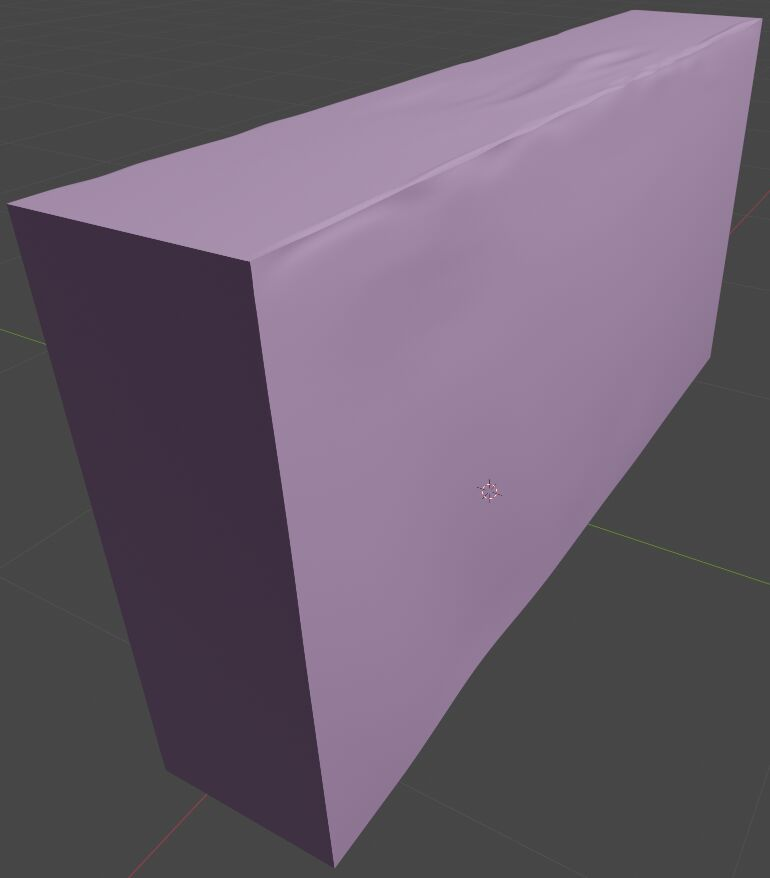
\includegraphics[width=0.4\textwidth]{imagenes/converted/barrier/barrierHP.jpg}
    \caption{Barrera de alta resolución con imperfecciones.}
    \label{fig:barreraHP}
\end{figure}

Como puede consumir demasiados recursos, he convertido las deformaciones geométricas en una textura normal utilizando Blender, de manera que se pueda poner sobre una versión simple de la barrera.

\begin{figure}[H]
    \centering
    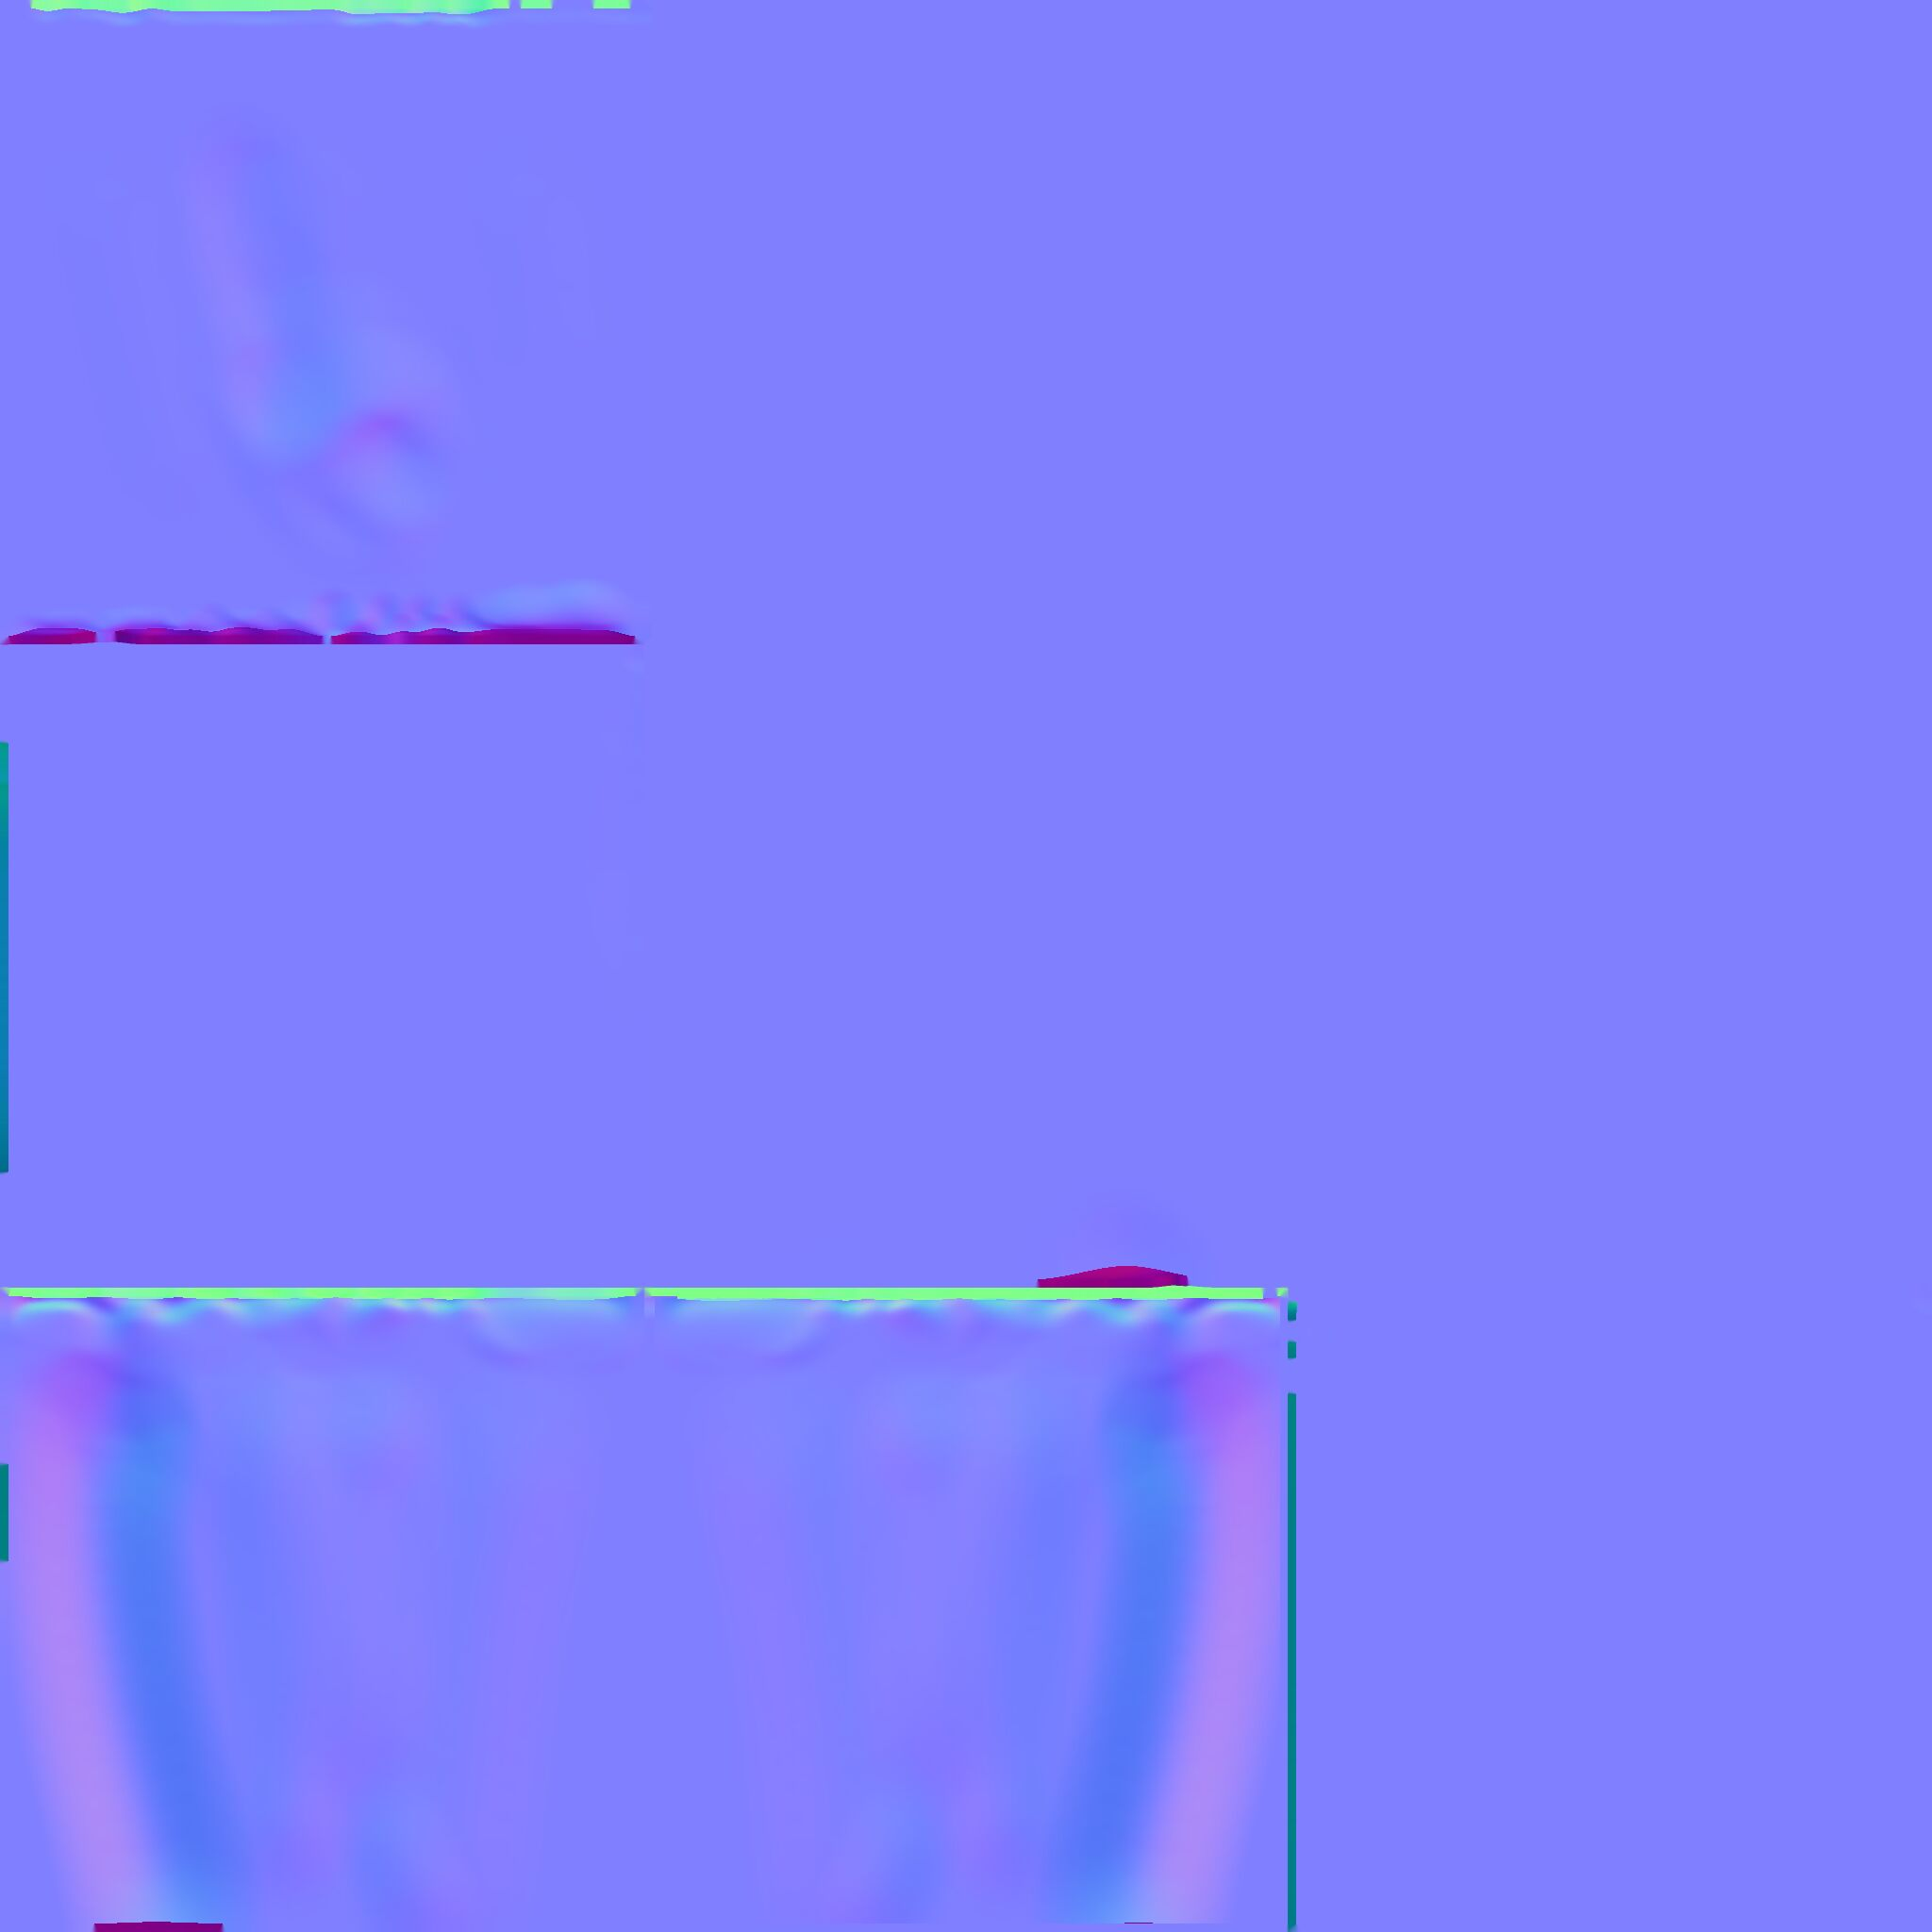
\includegraphics[width=0.4\textwidth]{imagenes/converted/barrier/barrierNormal.jpg}
    \caption{Textura normal generada para la versión con pocos polígonos.}
    \label{fig:barreraLP}
\end{figure}


Y el modelo final es mi barrera, junto a la valla anteriormente mencionada encima.

\begin{figure}[H]
    \centering
    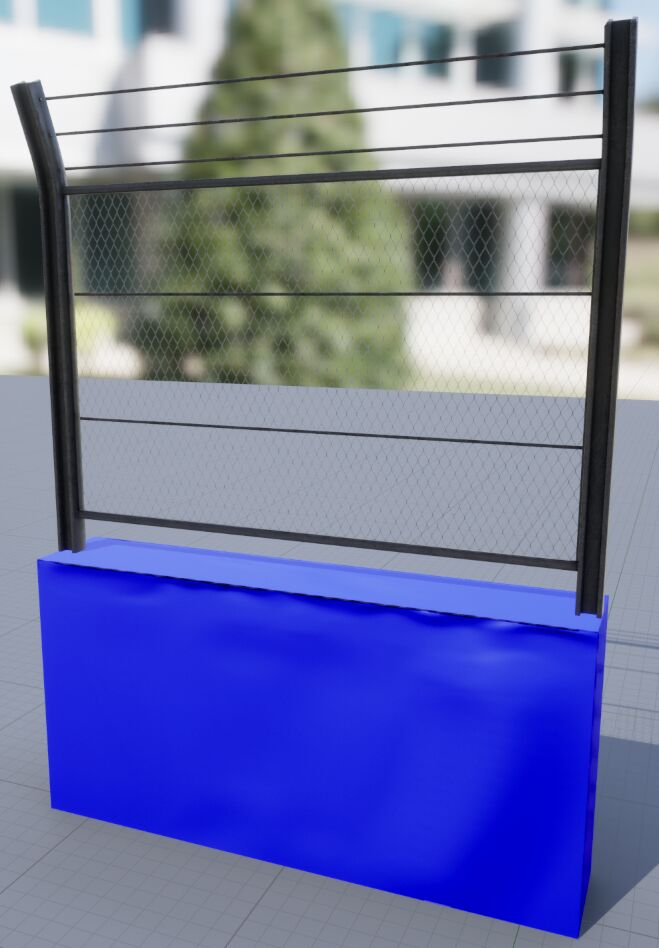
\includegraphics[width=0.4\textwidth]{imagenes/converted/barrier/barrierfence.jpg}
    \caption{Resultado final de la barrera en Unreal.}
    \label{fig:barreraFinal}
\end{figure}

Para que la barrera rodee todo el circuito, se sigue un procedimiento similar al del trazado. Se utiliza un spline que marca el recorrido y, luego, se asigna una barrera a cada sección del spline.

\newpage

\subsection{Vegetación}

La vegetación del circuito está compuesta por césped en el interior y exterior de las curvas y por árboles en el exterior y zonas intermedias del circuito. El modelo de césped utilizado ha sido ``temperate Vegetation: optimized Grass Library''\cite{grass}, creado por ``Project Nature'', y el de los árboles es ``Megascans Trees: European Black Alder (early access)''\cite{trees}, creado por ``Quixel Megascans''.

\bigskip

El resultado final es el siguiente:

% fotos de cerca de arboles y cesped
\begin{figure}[H]
    \centering
    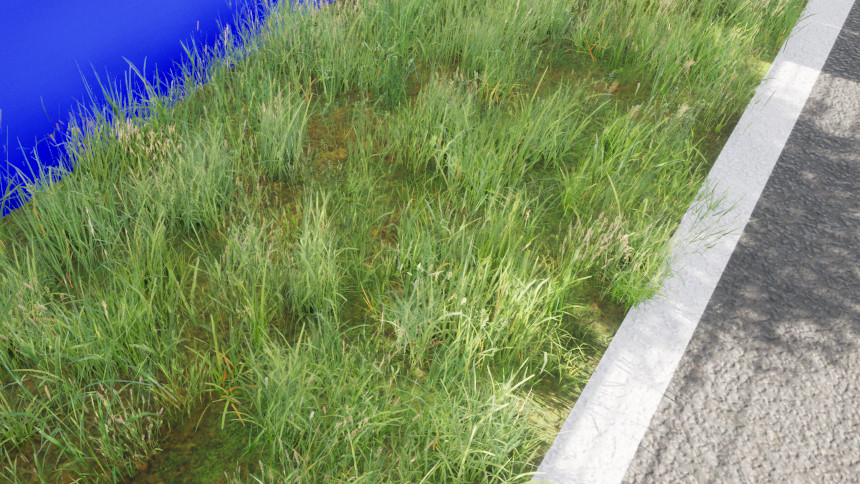
\includegraphics[width=0.9\textwidth]{imagenes/converted/cesped.jpg}
    \caption{Modelo de césped.}
    \label{fig:cesped}
\end{figure}

\begin{figure}[H]
    \centering
    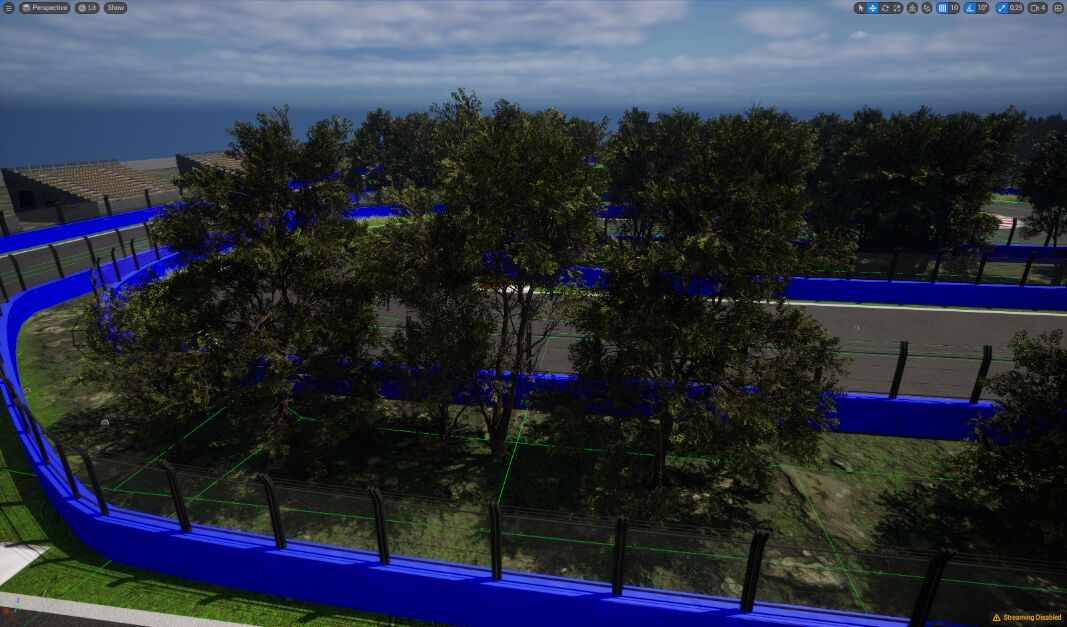
\includegraphics[width=0.9\textwidth]{imagenes/converted/arboles.jpg}
    \caption{Modelo de árboles.}
    \label{fig:arboles}
\end{figure}

\subsection{Modelos y texturas adicionales}

% rescribir
Adicionalmente, se ha utilizado la textura de césped ``Ground 037''\cite{grasstexture}, creada por ``Lennart Demes'', para las zonas en las que se puso el modelo tridimensional de césped (modelo 3D en figura \ref{fig:cesped}), con el objetivo de dar más realismo a distancias más alejadas, donde el modelo tridimensional no se aprecia.

\begin{figure}[H]
    \centering
    % \includegraphics[width=\textwidth]{imagenes/trazado.jpg}
    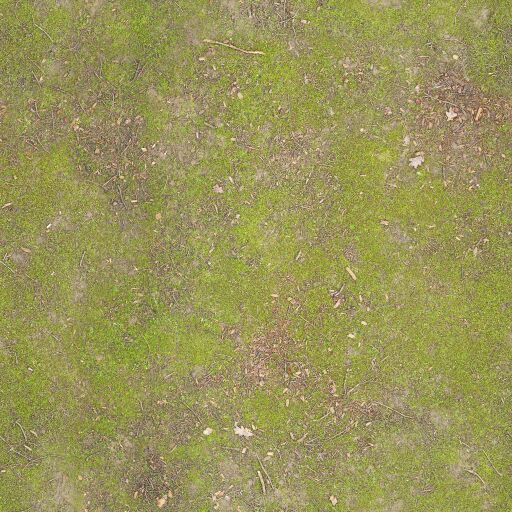
\includegraphics[width=0.4\textwidth]{imagenes/converted/Ground037_1K_Color.jpg}
    \caption{Componente difusa de la textura de césped utilizada.}
    \label{fig:grasstexture}
\end{figure}

Además, se ha hecho uso de la textura ``Coast Sand Rocks 02''\cite{coastsand}, creada por ``Rob Tuytel'', para el suelo del exterior del circuito, donde se encuentran los árboles (modelo 3D en figura \ref{fig:arboles}).

\begin{figure}[H]
    \centering
    % \includegraphics[width=\textwidth]{imagenes/trazado.jpg}
    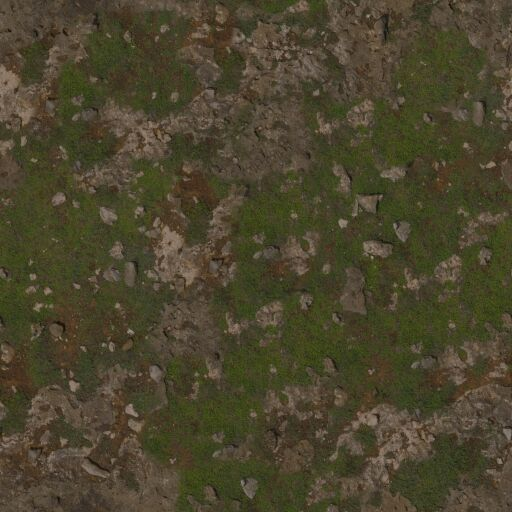
\includegraphics[width=0.4\textwidth]{imagenes/converted/coast_sand_rocks_02_diff_4k.jpg}
    \caption{Componente difusa de la textura del suelo.}
    \label{fig:coastsand}
\end{figure}

Por último, se ha utilizado el modelo ``Grand stand 3d model''\cite{grandstand}, creado por ``VT Studios'', para incluir algunas gradas en los alrededores del circuito.

\begin{figure}[H]
    \centering
    % \includegraphics[width=\textwidth]{imagenes/trazado.jpg}
    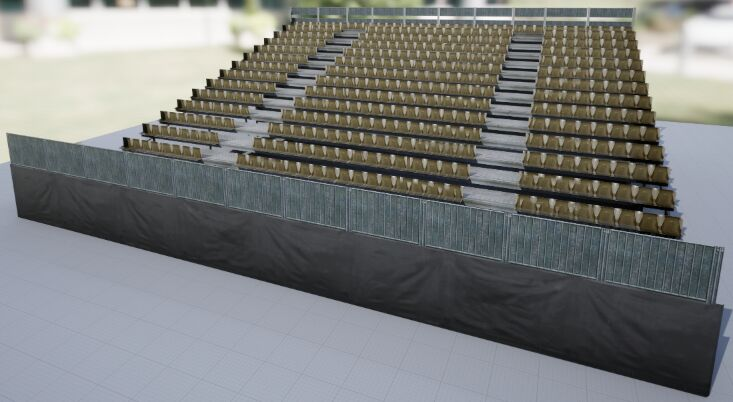
\includegraphics[width=\textwidth]{imagenes/converted/grandstand.jpg}
    \caption{Modelo de las gradas utilizadas.}
    \label{fig:grandstand}
\end{figure}